% Nicholas Wardle - Imperial College 
% nw709
\documentclass{mythesis}
\usepackage{mythesis}

\usepackage{rotating} % For making a sideways table
\usepackage{multirow} % For putting a header over more than 1 column
\usepackage{comment} % Allows you to comment out whole chunks of text
\usepackage{setspace}
\usepackage[numbers]{natbib}

\newcolumntype{A}{>{\centering\arraybackslash}p{1cm}} % allows you to centre columns
\newcolumntype{B}{>{\centering\arraybackslash}p{2cm}} % allows you to centre columns
\newcolumntype{C}{>{\centering\arraybackslash}p{3cm}} % allows you to centre columns
\newcolumntype{D}{>{\centering\arraybackslash}p{4cm}} % allows you to centre columns
\newcolumntype{E}{>{\centering\arraybackslash}p{5cm}} % allows you to centre columns
\newcolumntype{F}{>{\centering\arraybackslash}p{6cm}} % allows you to centre columns

% Custom commands -----------------------
%Theory
\makeatletter
\newcommand{\Rmnum}[1]{\expandafter\@slowromancap\romannumeral #1@}
\makeatother
%%%AlphaT%%%%%
\newcommand{\kfactor}{\ensuremath{k\text{-factor}}\xspace}
\newcommand{\kfactors}{\ensuremath{k\text{-factors}}\xspace}
\newcommand{\njet}{\ensuremath{n_{\text{jet}}}\xspace}
\newcommand{\njetlow}{\ensuremath{2 \leq \njet \leq 3}\xspace}
\newcommand{\njethigh}{\ensuremath{\njet \geq 4}\xspace}
\newcommand{\nb}{\ensuremath{n_{\text{b}}}\xspace}
\newcommand{\alphat}{\ensuremath{\alpha_{\text{T}}}\xspace}
\newcommand{\alphatcut}{\ensuremath{\alpha_{\text{T}}^{\text{cut}}}\xspace}
\newcommand{\htalphat}{\texttt{HT\_AlphaT}\xspace}
\newcommand{\htcat}{\ensuremath{\HT^{\text{cat}}}\xspace}
\newcommand{\photon}{\texttt{Photon}\xspace}
\newcommand{\muht}{\texttt{Mu\_HT}\xspace}
\newcommand{\httrigger}{\texttt{HT}\xspace}
\newcommand{\mt}{\ensuremath{M_{\textrm T}}\xspace}
\newcommand{\gj}{\ensuremath{\gamma} + jets\xspace}
\newcommand{\mj}{\ensuremath{\mu} + jets\xspace}
\newcommand{\mmj}{\ensuremath{\mu\mu} + jets\xspace}
\newcommand{\lj}{\ensuremath{\ell} + jets\xspace}
\newcommand{\llj}{\ensuremath{\ell\ell} + jets\xspace}
\newcommand{\ej}{\ensuremath{e} + jets\xspace}
\newcommand{\eej}{\ensuremath{ee} + jets\xspace}
\newcommand{\npre}{\ensuremath{N_{\textrm{pred}}}\xspace}
\newcommand{\nobs}{\ensuremath{N_{\textrm{obs}}}\xspace}
\newcommand{\njets}{\ensuremath{N_{\textrm{jet}}}\xspace}
\newcommand{\sq}{\ensuremath{\tilde{\rm q}}\xspace}
\newcommand{\st}{\ensuremath{\tilde{\rm t}}\xspace}
\newcommand{\gl}{\ensuremath{\tilde{\rm g}}\xspace}
\newcommand{\dht}{\ensuremath{\Delta\scalht}\xspace}
\newcommand{\dEt}{\ensuremath{\Delta\Et}\xspace}
\newcommand{\ewk}{\ensuremath{\mathrm{EWK}}\xspace}
\newcommand{\qcd}{\ensuremath{\mathrm{QCD}}\xspace}
\newcommand{\fZinv}[1]{\ensuremath{f_{\rm Zinv}^{#1}}\xspace}
\newcommand{\zInv}[1]{\ensuremath{Z_{\rm inv}^{#1}}\xspace}
\newcommand{\meanHt}[1]{\ensuremath{\langle \HT \rangle^{#1}}\xspace}
\newcommand{\lk}[2]{\ensuremath{L^{\rm #1}_{\rm #2}}\xspace}
\newcommand{\sep}{\ensuremath{68^{\mathrm{th}}}\xspace}
\newcommand{\partonht}{\ensuremath{\scalht^{\rm parton}}\xspace}
\newcommand{\meff}{\ensuremath{M_{\rm eff}}\xspace}
\newcommand{\mhttt}{\ensuremath{\hslash_{\rm T}^{TT}}\xspace}
\newcommand{\ifb}{\ensuremath{\text{fb}^{-1}}\xspace}
\newcommand{\ipb}{\ensuremath{\text{pb}^{-1}}\xspace}
\newcommand{\DMtt}{DM\ensuremath{+t\bar{t}}\xspace}
\newcommand{\DMj}{DM\ensuremath{+\rm{jet}}\xspace}
\newcommand{\DMbb}{DM\ensuremath{+b\bar{b}}\xspace}
\newcommand{\mchi}{\ensuremath{m_{\chi}}\xspace}
\newcommand{\mphi}{\ensuremath{M_{\Phi}}\xspace}
\newcommand{\pchi}{\ensuremath{\chi}\xspace}
\newcommand{\pphi}{\ensuremath{\Phi}\xspace}
\newcommand{\gsm}{\ensuremath{g_{\textrm{SM}}}\xspace}
\newcommand{\gdm}{\ensuremath{g_{\textrm{DM}}}\xspace}


%%%GENERIC%%%


\newcommand\rs{\raisebox{1.0ex}[-1.0ex]}
\newcommand{\ra}{\ensuremath{\rightarrow}}
\newcommand{\znunu}{\ensuremath{{\text Z} \ra \nu\bar{\nu}}\xspace}
\newcommand{\zll}{\ensuremath{{\text Z} \ra \ell\ell}\xspace}
\newcommand{\zmumu}{\ensuremath{{\text Z} \ra \mu\mu}\xspace}
\newcommand{\zee}{\ensuremath{{\text Z} \ra ee}\xspace}
\newcommand{\wmunu}{\ensuremath{{\text W} \ra \mu\nu}}
\newcommand{\wtaunu}{\ensuremath{{\text W} \ra \tau\nu}}
\newcommand{\dphi}{\ensuremath{\Delta \phi}}
\newcommand{\dphijj}{\ensuremath{\Delta \phi_{ j1,j2}}}
\newcommand{\pt}{\ensuremath{{p_{\text T}}}\xspace}
\newcommand{\pts}{\ensuremath{p_{\text T}{\text s}}\xspace}
\newcommand{\Et}{\ensuremath{{E_{\text T}}}\xspace}
\newcommand{\ptjf}{\ensuremath{p_{\rm T}^{ {\rm j}_1} }}
\newcommand{\ptjs}{\ensuremath{p_{\rm T}^{ {\rm j}_2} }}
\newcommand{\ptjt}{\ensuremath{p_{\rm T}^{ {\rm j}_3} }}
\newcommand{\etajf}{\ensuremath{\eta^{ {\rm j}_1} }}
\newcommand{\etajs}{\ensuremath{\eta^{ {\rm j}_2} }}
\newcommand{\etajt}{\ensuremath{\eta^{ {\rm j}_3} }}
\newcommand{\ttj}{\ensuremath{\rm{t}\bar{\rm{t}} + jets}\xspace}
\newcommand{\wj}{\ensuremath{\rm W + \textrm{jets}}\xspace}
\newcommand{\wej}{\ensuremath{{\rm W}(\rightarrow{\rm e}\nu) + \textrm{jets}}\xspace}
\newcommand{\wmj}{\ensuremath{{\rm W}(\rightarrow\mu\nu) + \textrm{jets}}\xspace}
\newcommand{\zj}{\ensuremath{{\rm Z} + \textrm{jets}}\xspace}
\newcommand{\zmmj}{\ensuremath{{\rm Z}(\rightarrow\mu\mu) + \textrm{jets}}\xspace}
\newcommand{\zeej}{\ensuremath{{\rm Z}(\rightarrow{\rm ee}) + \textrm{jets}}\xspace}

\newcommand{\al}{\ensuremath{\alpha}}
\newcommand{\alt}{\ensuremath{\alpha_{\text{T}}}\xspace}
\newcommand{\etaabs}{\ensuremath{|\eta|}}
%\newcommand{\gev}{\ensuremath{\mathrm{\,Ge\kern -0.1em V}}}
\newcommand{\pb}{\ensuremath{pb^{-1}}}
\newcommand{\mjj}{\ensuremath{M_{\text{inv}}^{j1,j2}}}
%\newcommand{\ttbar}{\ensuremath{t\bar{t}}}
\newcommand{\chiznew}{\ensuremath{\chi^{0}}\xspace}
\newcommand{\chipnew}{\ensuremath{\chi^{+}}\xspace}
%\newcommand{\chipm}{\ensuremath{\chi^{\pm}}\xspace}
\newcommand{\sQuanew}{\ensuremath{\tilde{\rm q}}\xspace}
\newcommand{\sGlunew}{\ensuremath{\tilde{\rm g}}\xspace}
\newcommand{\ttNew}{\ensuremath{\rm{t}\bar{\rm{t}}}\xspace}
\newcommand{\tev}{\TeV}
%<TW date="30/10/2010">
%\newcommand{\Et}{E_{T}}
\newcommand{\combIso}{Iso_{\textrm{comb.}}}
\renewcommand{\arraystretch}{1.2}
\newcommand{\bigNum}[2]{#1 \, \times \, 10 \, ^{#2}}
%</TW>

\newcommand{\raT}{\ensuremath{R_{\alt}}}
\newcommand{\RaT}{\ensuremath{R_{\alt}}\xspace}

\newcommand{\Ttwocc}{\ensuremath{\text{pp}\,\ra\,\sTop\sTop^{*}\,\ra\,\text{c}\chiz\,\bar{\text{c}}\chiz}}
\newcommand{\Ttwotc}{\ensuremath{\text{pp}\,\ra\,\sTop\sTop^{*}\,\ra\,\text{t}\chiz\,\bar{\text{c}}\chiz}}
\newcommand{\Ttwodegen}{\ensuremath{\text{pp}\,\ra\,\sTop\sTop^{*}\,\ra\,\text{b}ff'\chiz \,\text{b}ff'\chiz}}
\newcommand{\Ttwobw}{\ensuremath{\text{pp}\,\ra\,\sTop\sTop^{*}\,\ra\,\text{b}W\chiz \,\bar{\text{b}}W\chiz}}
\newcommand{\Ttwott}{\ensuremath{\text{pp}\,\ra\,\sTop\sTop^{*}\,\ra\,\text{t}\chiz\,\bar{\text{t}}\chiz}}
\newcommand{\Ttwobb}{\ensuremath{\text{pp}\,\ra\,\sBot\sBot^{*}\,\ra\,\text{b}\chiz\,\bar{\text{b}}\chiz}}
\newcommand{\Ttwoqq}{\ensuremath{\text{pp}\,\ra\,\sQua\sQua^{*}\,\ra\,\text{q}\chiz\,\bar{\text{q}}\chiz}}
\newcommand{\Tonebbbb}{\ensuremath{\text{pp}\,\ra\,\sGlunew\sGlunew^{*}\,\ra\,\bar{\text{b}}\text{b}\chiz\,\bar{\text{b}}\text{b}\chiz}}
\newcommand{\Toneqqqq}{\ensuremath{\text{pp}\,\ra\,\sGlunew\sGlunew^{*}\,\ra\,\bar{\text{q}}\text{q}\chiz\,\bar{\text{q}}\text{q}\chiz}}
\newcommand{\Tonetttt}{\ensuremath{\text{pp}\,\ra\,\sGlunew\sGlunew^{*}\,\ra\,\bar{\text{t}}\text{t}\chiz\,\bar{\text{t}}\text{t}\chiz}}
\newcommand{\Tonettbb}{\ensuremath{\text{pp}\,\ra\,\sGlunew\sGlunew^{*}\,\ra\,\bar{\text{t}}\text{t}\chiz\,\bar{\text{b}}\text{b}\chiz}}

\newcommand{\ppToGluGlu}{\ensuremath{\text{pp}\,\ra\,\sGlunew\sGlunew^{*}}}
\newcommand{\chipmToWNo}{\ensuremath{\chipm \,\ra\,W^{\pm}\chiz}}
\newcommand{\gluToBBNo}{\ensuremath{\sGlunew\,\ra\,\bar{\text{b}}\text{b}\chiz}}
\newcommand{\gluToTTNo}{\ensuremath{\sGlunew\,\ra\,\bar{\text{t}}\text{t}\chiz}}
\newcommand{\gluToQQNo}{\ensuremath{\sGlunew\,\ra\,\bar{\text{q}}\text{q}\chiz}}
\newcommand{\gluToTBAll}{\ensuremath{\sGlunew\,\ra\,\text{t}\text{b}\chipm(W^{\pm}\chiz)/\bar{\text{t}}\text{t}\chiz/\bar{\text{b}}\text{b}\chiz}}
\newcommand{\gluToTBWNo}{\ensuremath{\sGlunew\,\ra\,\text{t}\text{b}\chipm, \chipmToWNo}}
\newcommand{\gluToTStop}{\ensuremath{\sGlunew\,\ra\,\text{t}\sTop}}
\newcommand{\ppToStopStop}{\ensuremath{\text{pp}\,\ra\,\sTop\sTop^{*}}}
\newcommand{\stopToTNo}{\ensuremath{\sTop\,\ra\,\text{t}\chiz}}
\newcommand{\stopToCNo}{\ensuremath{\sTop\,\ra\,\text{c}\chiz}}
\newcommand{\stopToBWNo}{\ensuremath{\sTop\,\ra\,\text{b}\chipm,\chipmToWNo}}
\newcommand{\stopToBFFNo}{\ensuremath{\sTop\,\ra\,\text{b}ff'\chiz}}
\newcommand{\stopToMixed}{\ensuremath{\sTop\,\ra\,\text{c}\chiz/\text{b}ff'\chiz}}
\newcommand{\stopToTB}{\ensuremath{\sTop\,\ra\,\text{t}\chiz/\text{b}\chipm,\chipmToWNo}}
\newcommand{\stopToBW}{\ensuremath{\sTop\,\ra\,\text{b}\chipm,\chipmToWNo}}
\newcommand{\ppToSbotSbot}{\ensuremath{\text{pp}\,\ra\,\sBot\sBot^{*}}}
\newcommand{\sbottomToB}{\ensuremath{\sBot\,\ra\,\text{b}\chiz}}
\newcommand{\ppToSquaSqua}{\ensuremath{\text{pp}\,\ra\,\sQua\sQua^{*}}}
\newcommand{\squarkToQ}{\ensuremath{\sQua\,\ra\,\text{q}\chiz}}

\newcommand\T{\rule{0pt}{2.6ex}}
\newcommand\B{\rule[-1.2ex]{0pt}{0pt}}

\def\eslash{{\hbox{$E$\kern-0.6em\lower-.05ex\hbox{/}\kern0.10em}}}
\def\vecmet{\mbox{$\vec{\eslash}_T$}} %missing ET vector
\def\vecet{\mbox{$\vec{E}_\text{T}$}} % ET vector
\def\MET{\mbox{$\eslash_\text{T}$}\xspace}
%\def\met{\mbox{$\eslash_\text{T}$}\xspace}
\def\met{\mbox{$E_\text{T}^{\rm miss}$}\xspace}
\def\pfmet{\mbox{$\eslash_\text{T}^{\rm PF}$}\xspace}
\def\mex{\mbox{$\eslash_\text{x}$}} %missing Ex
\def\mey{\mbox{$\eslash_\text{y}$}} %missing Ey
\def\mepar{\mbox{$\eslash_\parallel$}}
\def\meperp{\mbox{$\eslash_\perp$}}
\def\Zmm{Z \rightarrow \mu\mu}
\def\metvec{\mbox{$\vec{\met}$}\xspace}
\def\metvecrec{\mbox{$\vec{\met}^{\rm rec}$}\xspace}
\def\metvecgen{\mbox{$\vec{\met}^{\rm gen}$}\xspace}
\def\metgen{\mbox{$\met^{\rm gen}$}\xspace}
\def\metparl{\mbox{$\mepar^{\rm rec}$}\xspace}
\def\metperp{\mbox{$\meperp^{\rm rec}$}\xspace}
\def\deltamet{\mbox{$\Delta\met$}\xspace}
\def\pthat{\mbox{$\hat{p}_T$}\xspace}
\def\hslash{{\hbox{$H$\kern-0.8em\lower-.05ex\hbox{/}\kern0.10em}}}
\def\MHT{\mbox{$\hslash_\text{T}$}\xspace}
%\def\mht{\mbox{$\hslash_\text{T}$}\xspace}
\def\mht{\mbox{$H_{\rm T}^{\rm miss}$}\xspace}
\def\mhtvec{\mbox{$\vec{H}_{\rm T}^{\rm miss}$}\xspace}
%\def\mhtmet{\mbox{$\hslash_\text{T} / \eslash_\text{T}$}\xspace}
\def\mhtmet{\mbox{$\mht / \met$}\xspace}
\def\mhtmetmiss{\mbox{$\H_\text{T}^{\rm miss} / \E_\text{T}^{\rm miss}$}\xspace}
%\def\rmhtmet{\mbox{$R_{\hslash_\text{T} / \eslash_\text{T}}$}\xspace}
\def\rmhtmet{\mbox{$R_{\mht / \met}$}\xspace}
\def\sumet{\mbox{$\sum \rm{E}_\text{T}$}\xspace}
\def\scalht{\mbox{$H_\text{T}$}\xspace}
\def\etmiss{\mbox{$\eslash_\text{T}$}\xspace}
\def\htmiss{\mbox{$\hslash_\text{T}$}\xspace}
\def\mtt{\mbox{$\rm{M}_\text{T2}$}\xspace}
\def\rmec{\mbox{$R_{\mht/\met}$}\xspace}
\def\bdphi{\mbox{$\Delta\phi^{*}_{\rm min}$}\xspace}
\def\dphimhtj{\mbox{$\Delta\phi(j_{1234}, \mht)_{\rm min}$}\xspace}
\def\dphimhtjall{\mbox{$\Delta\phi(j_{all}, \mht)_{\rm min}$}\xspace}
\def\bigeslash{{\hbox{$E$\kern-0.38em\lower-.05ex\hbox{/}\kern0.10em}}}
\def\bigmet{\mbox{$\bigeslash_T$}}
\def\bighslash{{\hbox{$H$\kern-0.6em\lower-.05ex\hbox{/}\kern0.10em}}}
\def\bigmht{\mbox{$\bighslash_T$}}
\def\incl{\includegraphics[width=0.49\linewidth]}
\def\inclrot{\includegraphics[angle=90,width=0.47\linewidth]}
\def\INCL{\includegraphics[angle=90,width=0.45\linewidth]}
\def\Incl{\includegraphics[angle=90,width=0.60\linewidth]}
\def\cls{\mbox{CL$_s$}\xspace}
\def\nj{\ensuremath{n_{\mathrm{jet}}}}
\def\nb{\ensuremath{n_{\mathrm{b}}}}

\newcommand{\zero}{\ensuremath{\phantom{0}}}



% ---------------------------------------
%% PDF metadata
\makeatletter
\@ifpackageloaded{hyperref}{%
\hypersetup{%
pdftitle = {},
pdfsubject = {},
pdfkeywords = {LHC, CMS, Higgs boson, Higgs to two photons, Combinations },
pdfauthor = {\textcopyright\ Nicholas Wardle}
}
}{}
\makeatother

% Define the thesis title and author
\title{Observation of a New Particle in the Search for the 
       Standard Model Higgs Boson at the CMS Detector}
\author{Nicholas Wardle}

% Start the document
%\bibliographystyle{unsrt}

\begin{document}
\pagenumbering{arabic}

% Define the un-numbered front matter (cover pages, rubrik and table of contents)
\begin{frontmatter}
\pagenumbering{arabic}
  %% Title
\titlepage[Imperial College London\\Department of Physics]%
{A dissertation submitted to Imperial College London\\
  for the degree of Doctor of Philosophy}

\clearpage
\textbf{The copyright of this thesis rests with the author and is made available under a Creative Commons 
Attribution Non-Commercial No Derivatives licence. Researchers are free to copy, distribute or 
transmit the thesis on the condition that they attribute it, that they do not use it for commercial 
purposes and that they do not alter, transform or build upon it. For any reuse or redistribution, 
researchers must make clear to others the licence terms of this work.}
%\clearpage


%% Abstract
\begin{abstract}%[\smaller \thetitle\\ \vspace*{1cm} \smaller {\theauthor}]
  %\thispagestyle{empty}
  The search for beyond standard model (BSM) physics is one of the primary physics objectives of the LHC.
  This thesis describes the~$\alpha_{\text{T}}$~search for supersymmetry using a dataset of $12.9\,\text{fb}^{-1}$ 
  collected during the 2016 proton-proton runs by the CMS detector. The search uses a final state 
  containing significant hadronic activity in the form of jets, missing energy and no leptons or photons.
  Dedicated dimensionless variables ensure that backgrounds with fake missing energy are mitigated. A detailed description 
  is given of both the selections used to mitigate backgrounds while maintaining signal acceptance to a wide range of models and of
  the techniques used to ensure a robust determination of the residual backgrounds and systematic uncertainties.
  No evidence for BSM physics is observed and simplified models are therefore used to interpret the results of 
  the search. Stringent new limits are placed on a range of supersymmetric topologies and a procedure presented
  to allow the search to be re-interpreted for any BSM physics model.

  Additionally, the upgrade of the Level-1 trigger jet and energy sum algorithm
  is studied. The upgraded trigger hardware is exploited to ensure effective performance in conditions exceeding 
  the design specification of the LHC.

\end{abstract}


%% Declaration
\begin{declaration}
I, the author of this thesis, hereby declare the work contained in this 
document to be my own. All figures labelled `CMS' are sourced directly from CMS publications, 
including those produced by the author and have been referenced as such 
in the figure caption. Figures marked `CMS Preliminary' are sourced from an unpublished 
or preliminary public document. All figures and studies taken from external sources are referenced appropriately 
throughout this document.

The studies for the trigger upgrade presented in Chapter~\ref{cha:triggerUpgrade} are 
the result of my own work carried out within the UK CMS Trigger group. I have
been a major contributor to all areas of the $\alpha_\text{T}$ 
analysis presented in Chapters~\ref{cha:alphat}, \ref{cha:backgroundPrediction}, 
and \ref{cha:statisticalResults} as part of the Imperial College London and CERN SUSY groups.
The aspects of the search for which I have been particularly responsible are 
the inclusion of the \mht~shape described in Section~\ref{sec:syst-on-shape} 
and the statistical interpretations described in Chapter~\ref{cha:statisticalResults}.
Finally, I have carried out the work to facilitate re-interpretations described in 
Chapter~\ref{cha:simplifiedLikelihood} with a CMS collaborator.
%  \vspace*{1cm}
  \begin{flushright}
    Matthew Citron
  \end{flushright}
\end{declaration}


%% Acknowledgements
\begin{acknowledgements}
kthanksbye
\end{acknowledgements}


%% Preface
%\begin{preface}
% Insert preface here...
%\end{preface}

%% ToC
\tableofcontents

\listoffigures
\listoftables
%% Strictly optional!
\frontquote%
  {I struggled with some demons\\ They were middle class and tame}
  {Leonard Cohen}

\end{frontmatter}

%\doublespacing
%$ Start the content body of the thesis
\begin{mainmatter}
% Chapter 2

\chapter{The LHC and CMS experiment} % 
\section{The Large Hardon Collider}
%LHC intro 
The LHC is a 27km circular circumference storage ring, accelerator and collider for 
both protons and Pb ions. It is situated in a stable environment in a tunnel 
100 metres underneath the Franco-Swiss boder near Geneva, Switzerland.
A double-ring synchotron, it is designed to collide proton-proton (p-p)
pairs with a centre of mass energy of up to $\sqrt(s)=14\TeV$ and a 
luminosity of up to $10^{34}cm^{-2}s^{-1}$. This makes the LHC the only collider
in operation able to directly probe the $\TeV$ scale physics. 

The injected beams in the LHC are accelerated and stored for each physics run using 
a $400MHz$ superconducting cavity system. The beams of protons or pB ions 
are merged at four sections around the ring to enable collisions at interaction points.
At each of these four interaction points lies one of the four main 
experiments at the LHC; A Large Ion Collidor Experiment (ALICE) \cite{ALICE},
A Toroidal LHC Apparatus (ATLAS) \cite{ATLAS}, the Compact Muon solinoid (CMS) \cite{CMS}
and LHCb which record the collisions. Figure~\ref{LHC-diagram} shows the layout of the LHC ring including
the positions of the four main detectors. The proton beams are made up of many 'bunches' of approximately $1.1\times10^{11}$
protons localised into less than 1 ns in the direction of motion.
The beams are formed inside the Proton Synchrotron (PS) from bunches of protons 25 or 50 ns apart with an energy of 26 GeV. 
The protons are then accelerated in the Super Proton Synchrotron (SPS) to 450 GeV before being injected into the LHC at
the points shown in Figure~\ref{LHC-diagram}. Once injected into the LHC, Radio Frequency (RF) cavities 
provide around 275kW of RF power independently to each beam to accelerate the protons to allow collisions
at the operating centre of mass energy. For the work contained in the thesis $\sqrt(s) = 13\TeV$ with bunch spacings of both
25ns and 50 ns \cite{LHC}. The LHC operates as a storage ring for the accelerated beams using 1232 
superconducting dipole magnets in the eight arc segments which provide magnetic fields of up to $8T$ to steer the beams. 
High precision quadropole and higher order magnets at the interacton points are used to position and focus the beams to 
maximise the occurance of high momentum p-p collisions. The average number of simultaneous collisions
per bunch crossing, in time pile-up (PU), for the work in this thesis was $\approx25$.
The luminosity in the LHC is not constant over a physics run, but decays due to the degradation 
of intensities and emittances of the circulating beams (mainly due to loss from collisions). Eventually,
the beam is dumped and the acceleration process is started again. The turn around time between dumping
the beam and the start of a new physics run is typically around 6 hours.

\begin{figure}
\centering
    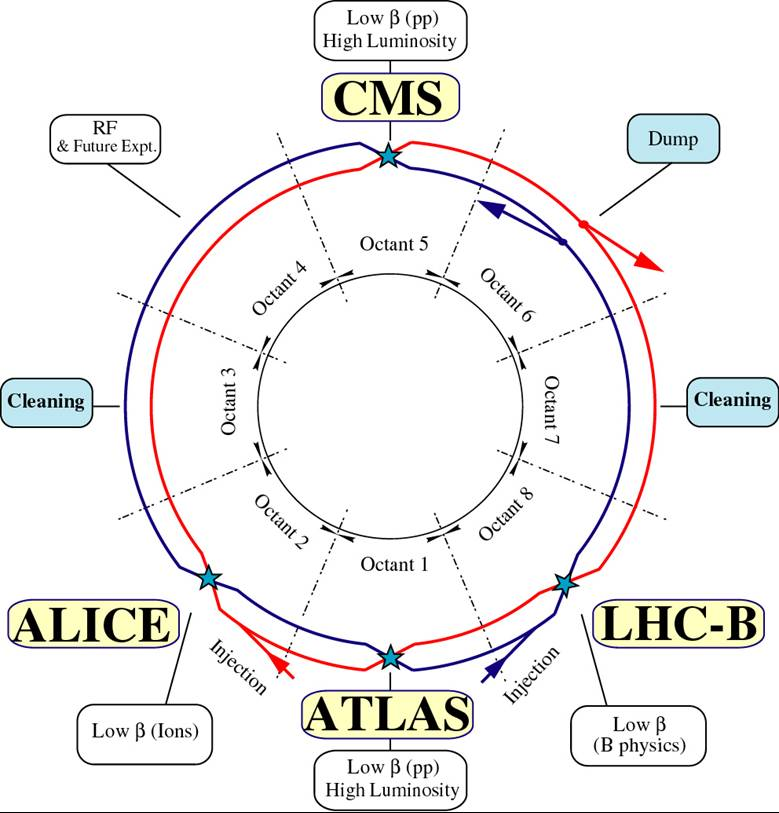
\includegraphics[width=0.8\textwidth]{./Figures/detector/lhcDiagram}
  \caption{Schematic layout of the LHC showing the position of the four main detectors as
  well as the RF systems}
  \label{fig:LHC-diagram}
\end{figure}

\subsection{LHC run condictions}

The first physics runs of the LHC from 2010-2013 (Run 1) reached energies of 3.5 and 4 TeV per beam and 
provided record-breaking integrated luminosities. The data collected allowed 
for the discovery of the higgs boson\cite{higgs} as well as enabling many new regions of parameter space
to be probed. From 2013 to mid-2015 (Long Shutdown 1) the LHC was shut down for upgrade to allow design
energies to be reached. All magnet interconnectors were inspected and replaced where necessary 
and the dipole magnets underwent a quench training programme. 

After LS1, from 2015-2016 (Run 2, which will continue up to 2018) the LHC has been running with record beam energies 
of $6.5\TeV$ per beam with bunch spacings of 25 and 50 ns. 
As shown in Figure~\ref{fig:LHC-integrated-lumi}, in 2016, $40.7\fb$ of integrated luminosity has been 
delivered to the CMS and ATLAS detectors, with $37.5\fb$ recorded by CMS. The dataset is validated by detector
subsytem experts to ensure runs in which the data quality may be affected by any problem in one of the CMS detectors 
subsystems are excluded. The luminosity of this certified dataset is XX and it is this dataset, 
at a centre of mass energy of $\sqrt(s) = 13\TeV$, 
which is used in Chapters XX to search for Supersymmetry at the highest energy reached at a collider.

%%%FIGURE - LHC lumi plot!
\begin{figure}
\centering
    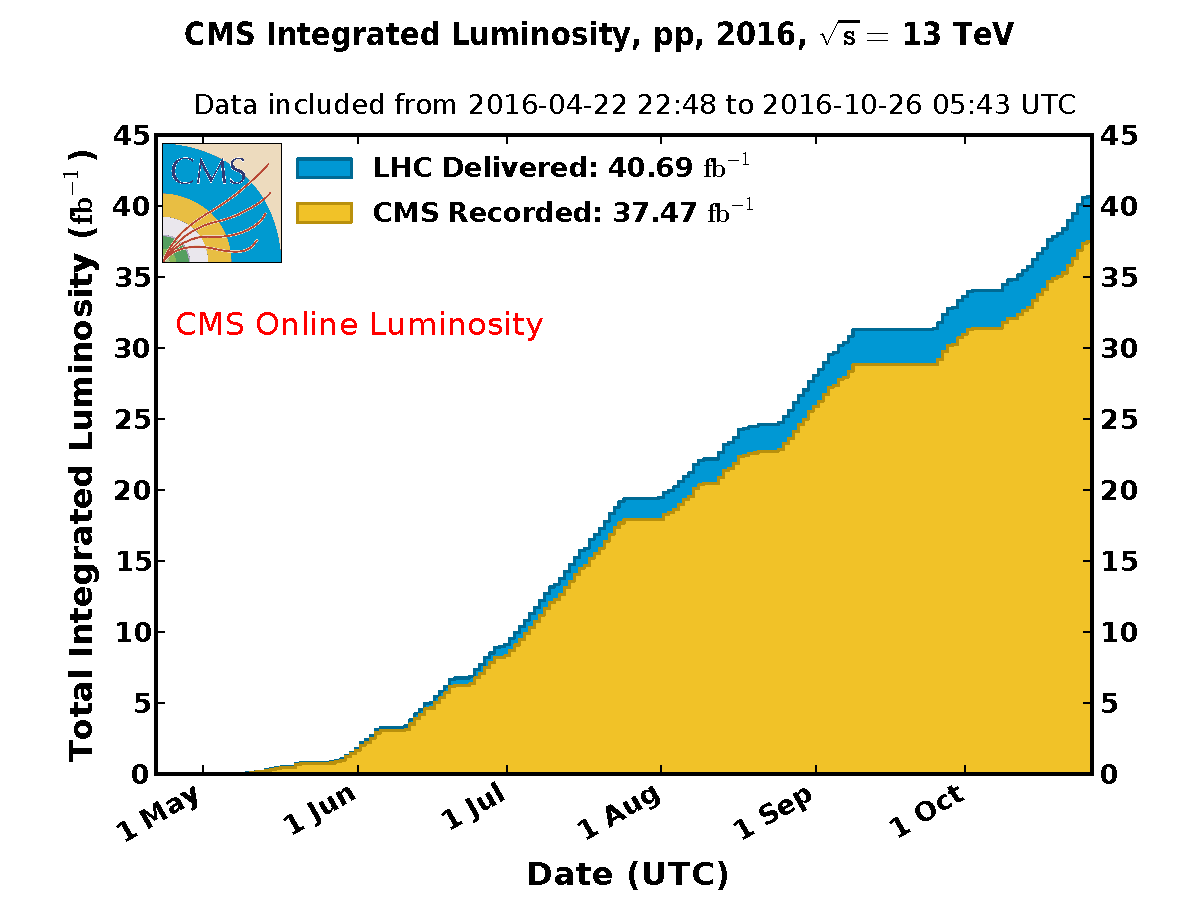
\includegraphics[width=0.9\textwidth]{./Figures/detector/int_lumi_per_day_cumulative_pp_2016OnlineLumi}
  \caption{Integrated luminosity measured online versus day delivered to (blue), 
  and recorded by CMS (orange) during stable beams and for p-p collisions at 13 TeV centre-of-mass energy in 2016.}
  \label{fig:LHC-integrated-lumi}
\end{figure}

%----------------------------------------------------------------------------------------
\section{The CMS detector}
The Compact Muon Solenoid (CMS \cite{CMS}) is one of two general purpose detectors at the LHC 
which have performed exceptionally well during the physics runs of the LHC. It was designed
with the aim of discovering the Higgs boson as well as searching for generic models 
of new physics. To achieve this, CMS provides efficient identification and measurement
of physics objects including muons, electrons, photons, taus and hadronic showers over a
wide range of momenta and energies and covering almost $4\pi$ in solid angle. 
Its traditional barrel design allows global momentum imbalance to be effectively 
reconstructed allowing the $\met$ predicted in many new models of physics to be
precisely measured. A more detailed description may be found in \cite{CMS}. 

\begin{figure}
\centering
    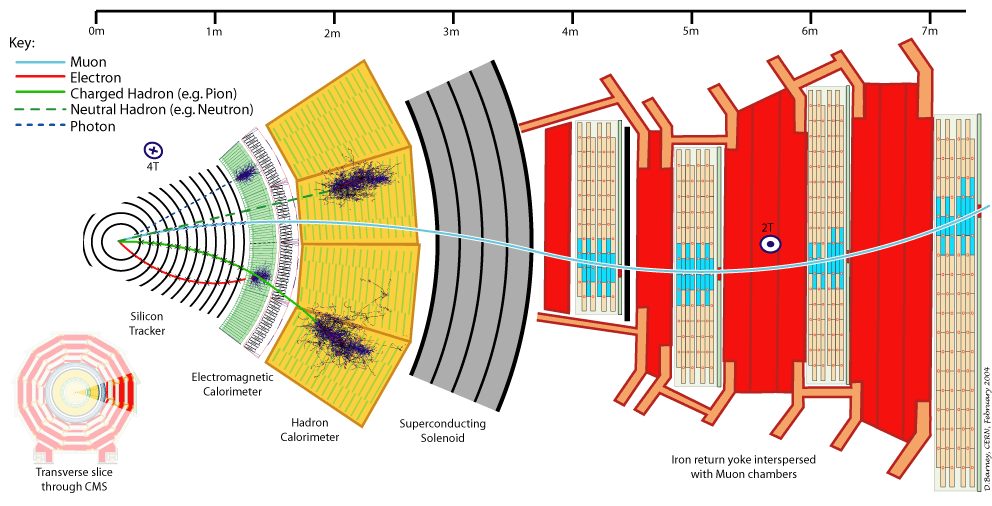
\includegraphics[width=0.9\textwidth]{./Figures/detector/CMS_Slice.jpg}
  \caption{Cross Section of CMS showing the paths of various particle types 
  through different segments of the detector \cite{cmsslice}}
  \label{CMS_SLICE}
\end{figure}

A cross section of CMS is shown in figure \ref{CMS_SLICE}. The coordinate system used by CMS takes the origin at 
the collision point. The z-axis points along the beam direction and defines the azimuthal angle, $\phi$. 
Instead of the polar angle, $\theta$, the psuedorapidity, $\eta=-ln(tan(\theta/2))$, is used as $\Delta \eta$
between two particles is approximately relativistically invariant. The eta coverage of CMS is $|\eta|<5$. 
Transverse energies and momenta ($E_T $ and $p_T$)  are defined perpendicular to the beam \cite{cmsiop}. 
The different detector components shown in figure \ref{CMS_SLICE} will now be described in detail. 
Resolutions are quoted for measuring the relevant property for a 100 GeV particle/jet \cite{SACharacteristics}.
\begin{description}
\item[Silicon Tracker]The job of the tracker is to measure the momentum of charged particles from their path through a magnetic field \cite{siliconTDR}. The CMS tracker achieves $10\mu m$ accuracy with coverage for $|\eta|<2.5$ and has a resolution of 1\%.
\item[Electromagnetic Calorimeter (ECAL)] The ECAL measures the energy of incident photons and electrons. The ECAL barrel is made of 61,200 $PbWO_4$ crystals and provides coverage for $|\eta|<1.48$ \cite{ecal}. This is extended to $|\eta|<3$ by the endcap which adds another $10764$ crystals. The endcap has a pre-shower to distinguish between $\gamma$ and $\pi^0$. The ECAL has a resolution of 0.5\%.
 \item[Hadronic Calorimeter (HCAL)] The HCAL is made from alternating brass and scintilator layers with a coverage of $|\eta|<3.0$ \cite{hcal}. The coverage is extended to  $|\eta|<5.0$ by an iron/quartz forward calorimeter \cite{hfhcal}. The average resolution is 11\%. 
 \item[Muon Chambers]The muons are not stopped by any of the calorimeters and therefore require a separate detector with coverage $|\eta| < 2.4$. The muon chambers are interspersed with the magnet return yoke. The high magnetic field allows for accurate momentum measurement \cite{muons}. The resolution is 1\%.
\end{description}
As the data rate ($40Mhz$) is far too high for every event to be stored and as new physics will only 
be seen in a minority of events a trigger system for interesting events is necessary. 
This happens in two stages: the L1 Calorimetric and Muon Trigger (Hardware) and the High Level Trigger (Software) \cite{HLT}. 
The L1 trigger must operate within $\mathcal{O}10ns$ and so  the calorimetric trigger only takes input
from the ECAL and HCAL. This is described in more detail in chapter \ref{Chapter3}. The input from the
L1 triggers is then combined in the Global Trigger (GT) which decides whether to keep the event. 
The $\mathcal{O}100kHz$ events which pass L1 selection are processed in the HLT which utilises the 
calorimeter information along with tracking and the muon system to further reduce the rate to $\mathcal{O}1kHz$.

\chapter{Reconstruction} % 
\label{cha:reco}

The precise measurement of particles produced in the high energy collisions at the LHC 
is necessary to effectively execute the CMS physics programme. This requires high precision
reconstruction and identification of physics objects in a challenging environment containing
large numbers of different particles with a range of energies. The \alphat analysis 
relies directly on reconstruction of jets and \met for the signal region and on the 
reconstruction of leptons and photons to reject electroweak 
backgrounds and to define control regions.
This requires the use of information from all detector subsystems and state-of-the-art
techniques to allow the reconstruction, selection and calibration of these physics objects.


\section{Detector reconstruction}

The first stage in reconstructing the physics objects is to produce the necessary
input information from the detector subsystems. This information may be tracks
(trajectories) of charged particles or energy measurements from calorimeter depositions. 
Specialist algorithms which suppress backgrounds, mitigate the effects of pileup and provide high resolution energy,
position and/or temporal measurements are used to optimise the precision of the 
measured quantities over a wide range of particle energies and momenta.

\subsection{Track reconstruction}

Charged particle tracks are reconstructed from the hits, considering the efficiency and resolution, 
using the iterative Combinatorial Track Finder (CTF) algorithm. The track reconstruction can be decomposed 
into four logical steps outlined below.

\begin{itemize}
\item Seeds are generated using either triplets of tracker hits or pairs of hits with an additional constraint 
from the beamspot or a pixel vertex. This gives an initial estimate of the trajectory with uncertainty~\cite{tracker_early}.
\item Each seed is propagated outward through the tracker layers while considering the current uncertainty in the trajectory.
In propagating, a uniform magnetic field is assumed as well as no energy loss or multiple Coulomb scattering effects.
The track parameters are updated with the best matching hit on each layer (if any) according to the Kalman filter formalism~\cite{tracker_vertex}.
The search continues until either the boundary of the tracker is reached or no more compatible hits are found. If a minimum number
of valid hits are observed an inwards search is initiated for additional hits~\cite{tracker_early}.
\item It is possible for a single charged particle track to be reconstructed more than once, starting either from different seeds or if
one seed develops into multiple track candidates. If the fraction of shared hits between two track candidates is greater
than 19\% (determined empirically) the track with fewer hits is discarded. If the number of hits is equivalent the track with
 the largest $\chi^2$ is discarded~\cite{tracker_vertex}.
\item After the track candidates are built and cleaned the hits in each candidate are refitted using a Kalman filter and smoother. This 
avoids possible bias from the seeding stage~\cite{tracker_vertex}.
\end{itemize}

The CTF performs six iterations to determine the tracks. Between each iteration any hits that are assigned to tracks in the
previous iteration are removed from the collection. The final track collection is then filtered to remove fake tracks using 
information on the number of hits, the $\chi^2$ and the compatibility of the track originating from a pixel vertex. The momentum 
resolution achieved is 0.7 (5)\% at 1 (1000) \GeV~in the central region~\cite{tracker_early}. Using a dataset of pions and muons from an early run 
at the LHC the tracking efficiency was measured as 98\% for tracks with $\pt > 500\MeV$ and $>99\%$ for tracks with $\pt > 2\GeV$\cite{tracker_eff}.

\subsection{Vertex Reconstruction}

As described in Section~\ref{lhc_intro}, the LHC produced an average of 25 simultaneous collisions per bunch crossing
during Run 2. It is essential to identify the Primary Vertex (PV) and the particles originating from it to allow 
particles from additional collisions to be rejected and to identify features such as displaced vertices. The tracks
are initially clustered using a deterministic annealing (DA) algorithm based on the points of closest approach of the 
tracks to the beamspot~\cite{tracker_vertex}. The candidate vertices containing at least two tracks are then
fitted using an adaptive vertex fitter (AVF) to compute the best estimates of vertex parameters~\cite{tracker_avf}. 
Each track in the vertex is assigned a weight between 0 and 1 corresponding to the likelihood that that track
belongs to the vertex. The tracks with weight near 1 are most consistent with the reconstructed vertex while
those that are least consistent have small weights. The number of degrees in the fit, defined as 

\begin{equation}
n_{dof} = -3 + 2 \sum_{i=1}^{\#tracks} wi,
\end{equation}

is an important parameter for distinguishing real proton-proton interactions from misclustered vertices as it is strongly corrected with
the number of tracks compatible with arising from the interaction region~\cite{tracker_vertex}. The vertex
position and resolution determined using the AVF have been 
measured in early LHC data and compared with simulation as shown in Fig~\ref{fig:pvEffRes}.

\begin{figure}[hbt]
  \begin{center} 
   \subfigure[\label{fig:pvEff}]{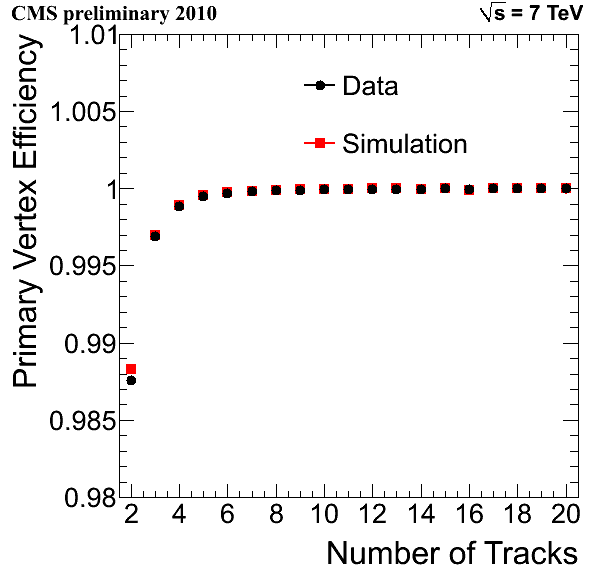
\includegraphics[width=0.5\textwidth]{Figures/detector/pvEff}}~
   \subfigure[\label{fig:pvRes}]{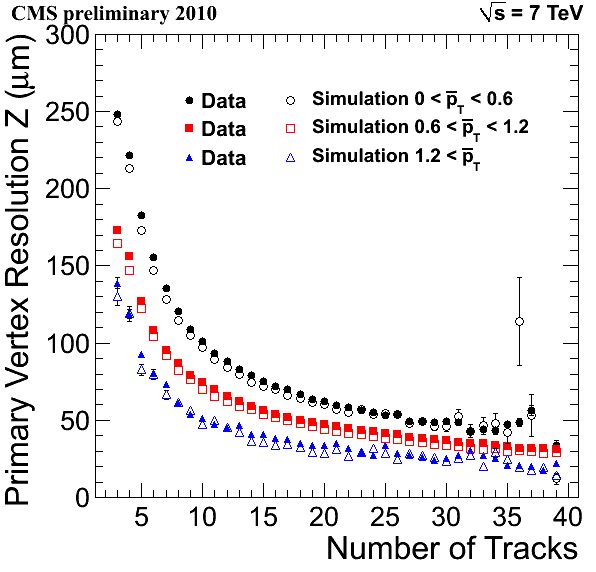
\includegraphics[width=0.5\textwidth]{Figures/detector/pvRes}}
   \caption{(a) Primary Vertex efficiency as a function of the number of associated tracks. (b) Primary Vertex 
   resolution in the z coordinate as a function of the number of associated tracks for three track \pt~scenarios~\cite{tracker_seven}
   \label{fig:pvEffRes} }
  \end{center}
\end{figure}

The vertices are ordered according to the sum of the $p_T^2$ of the tracks associated to each vertex with the 
vertex with the highest $p_T^2$ taken as the primary vertex (PV). The position of the primary vertex can
be used for object identification and control of pile-up. Many CMS analyses, including the one in this 
thesis, make requirements that a good vertex is reconstructed from the tracks satisfying:

\begin{itemize}
\item A minimum number of degrees of freedom: $n_{dof} > 4$.
\item The collision to occur with $|z| < 24cm$ such that the primary vertex is near the 
interaction point in the longitudinal direction.
\item The collision to occur within a radial distance of $|d_{xy}| < 24cm$ from the beamline.
\end{itemize}

\subsection{Calorimeter reconstruction}

The calorimeters reconstruct the energies of incident particles from deposits made in the 
various subsystems. These deposits must be clustered and the measurement calibrated to provide 
details of the energy, position and timing of the incident particle.
For neutral particles the calorimeter subsystems provide the only measurement of
the particle properties. For charged particles the measurement complements that
from the tracker and provides necessary redundancy in the case of track
misreconstruction.

The ECAL crystals are calibrated with both absolute and relative calibrations. Nine EB superclusters
and 500 EE crystals are calibrated using high energy electron beams to achieve a 
resolution of 0.5\% (1\%) for the EB (EE) components~\cite{ecal_calib}. 
The remainder undergo relative intercalibrations to achieve a resolution of 1.4\%-1.8\% ($\sim5\%$) 
for the EB (EE) components. During LHC runs the response of the crystals changes due to 
radiation induced crystal-lattice defects which absorb the scintillation light. 
The crystal transparency is monitored to allow the impact on energy measurements to
be assessed and corrected~\cite{ecal_calib}. 

The HCAL components undergo a similar calibration to the ECAL crystals. Firstly a subset of the 
components are calibrated with a 50 \GeV~pion beam which is then extended to the remainder of the 
subsystem using a Co source~\cite{hcal_beam}. Additional corrections
for the HCAL component are derived during LHC running~\cite{hcal_calib}.

The reconstruction of the energy at the HCAL and ECAL relies on recording the amplified 
light pulses from the photodiodes over a 25ns time sample. When operating with 25ns bunch 
spacing, particle energies from previous or following bunch crossings can be integrated
into this sample, biasing the energy measurement. This effect is correcting by using a 
dedicated reconstruction that removes the contributions from such Out Of Time Pileup 
(OOTPU)~\cite{hcal_timing,ecal_timing}. The 25ns sample is fitted including three pulse 
shape templates with variable amplitude and arrival times with the central pulse corresponding 
to the triggered event. The timing distribution for the ECAL hits above 1~\GeV, which is derived 
independently from the energy measurement, is shown in Figure~\ref{fig:timing_barrel_linear} 
showing the effective rejection of contributions from OOTPU.

\begin{figure}
\centering
    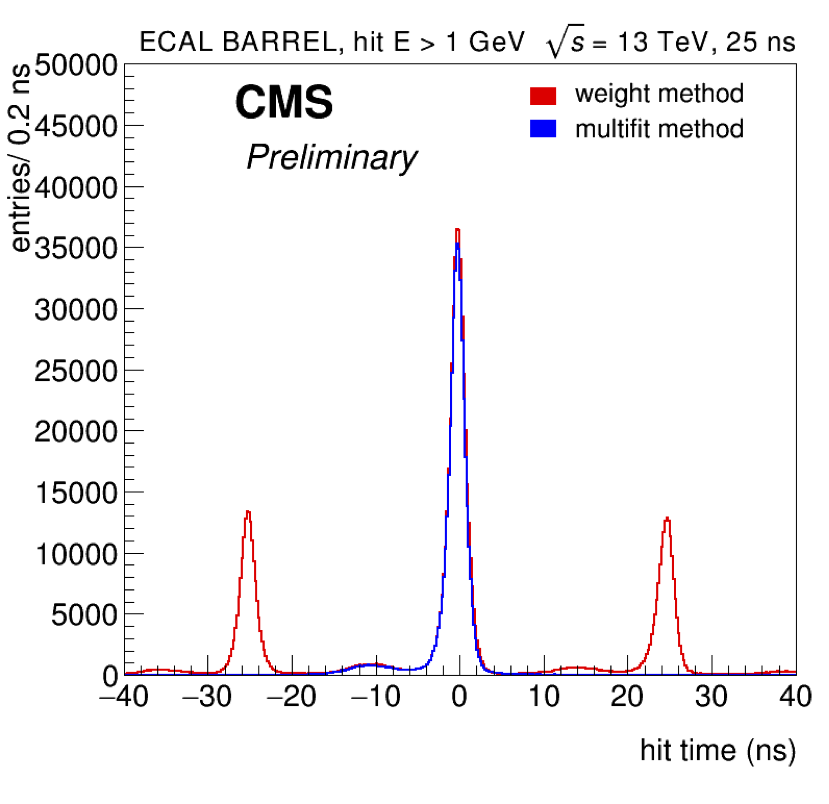
\includegraphics[width=0.8\textwidth]{./Figures/reconstruction/timing_barrel_linear.png}
  \caption{Timing distribution of the hits in the ECAL barrel with a reconstructed energy above 1\GeV~\cite{ecal_timing}.}
  \label{fig:timing_barrel_linear}
\end{figure}

\section{Physics object reconstruction}

The reconstructed tracks and calorimeters form the inputs to the reconstruction of the particles and 
jets that form the basis of the final selection of many analyses, including the analysis described 
in the thesis, referred to as physics objects. These are reconstructed using a combination of
dedicated local reconstruction algorithms as well as the global event Particle
Flow algorithm, described in Section~\ref{sec:particle_flow}.
In addition, several WPs of selection criteria are defined for each physics object 
which provide a range of efficiencies and corresponding proportion of false positives. 

\subsection{Electron and photon reconstruction}
\label{sec:ele_pho_reco}

Photons and electrons interact similarly within the ECAL and so these objects 
follow similar reconstruction techniques. Electrons are reconstructed by matching 
information in the tracker and ECAL using two complementary techniques, an ECAL driven 
reconstruction described in this section (identical, aside from tracking
requirements, to the photon reconstruction) and a tracker-driven reconstruction performed with
the PF algorithm (see Section~\ref{sec:particle_flow}) which is optimal for low \pt~electrons. 

In the ECAL, both electron and photon candidates are formed by clustering energy deposits
from electromagnetic showers. Around 50\% of the photons convert into an electron-positron 
pair in the material proceeding the calorimeter leaving an energy deposit that is widely 
spread in $\eta$ and $\phi$~\cite{electron_photon_reco}.  For unconverted photons the 
deposits are fairly localised in $\eta$ and $\phi$. Electrons radiate
bremsstrahlung along their trajectories due to the presence of the magnetic field and 
lose $33\%$ of their energy on average in the central region 
and up to $86\%$ at $|\eta| = 1.4$. Their energy deposits are widely spread in $\phi$ but narrow in $\eta$. 
The hybrid (multi) clustering algorithm exploits this characteristic to
reconstruct high energy electrons and photons in the barrel (endcap). The hybrid algorithm
uses a seed crystal and clusters up to ten \emph{dominoes} of $1\times3$ or $1\times5$ ($\phi\times\eta$) within 
$\Delta\phi < 0.3$ from the seed. Any domino with an energy under $100\MeV$ is discarded. The dominoes
are themselves clustered in $\phi$ provided each disconnected subcluster has a seed 
domino of energy $>350\MeV$. The combination of these subclusters is referred 
to as a supercluster. The reconstruction in the endcap follows a similar procedure 
using $5\times5$ grids of crystals. 

Superclusters which can be associated to tracks originating from the primary vertex are reconstructed as electrons.
As electrons lose energy through the non-Gaussian bremsstrahlung process the Kalman filter is inappropriate and
so the specialist track reconstruction Gaussian Sum Filter (GSF) algorithm is used. This allows the total energy of
electrons to be reconstructed including the component lost through bremsstrahlung. The photons are identified 
through inverting the track matching criteria of the supercluster. In the endcaps, additional information
is used from the preshower when reconstructing the energy.

Additional selections are applied on all reconstructed electrons and photons to suppress backgrounds.
For electrons these are mainly composed of misreconstructed jets, secondary electrons from photon
conversions and semi-leptonic decays of heavy quarks. As electrons are mainly contained within 
the ECAL, a requirement on the ratio of energies in the ECAL and HCAL provides a strong veto of hadronic
backgrounds. In addition, requirements are made on the matching track \emph{impact
parameters} such that the transverse distance from the primary vertex is $d_{xy} < 0.0261$ ($d_{xy} < 0.118$) 
and the longitudinal distance is $d_z < 0.041$ ($d_z < 0.822$) for the barrel (endcap). 
Several variables that rely on the shower shape and cluster width are used to
reject fakes, including $\sigma_{i\eta i\eta}$ (the second moment of the log-weighted
distribution of crystal energies calculated in the $5\times5$ matrix around the
most energetic crystal). The value of $\sigma_{i\eta i\eta}$ allows background
processes to be rejected as its value is larger on average for neutral meson decay to two collimated photons.

\subsection{Muon reconstruction}
\label{sec:muon_reco}

As muons are MIPs they leaving minimal energy deposits in the calorimetry
subsystems and travel through the entire detector. The muons are therefore reconstructed using a 
combination of the inner tracker and muon systems. Two algorithms are used to 
give complementary efficiency across the momentum spectrum, the 'the outside-in' 
global muon algorithm and 'the inside-out' tracker muon algorithm~\cite{muon_reco}.

The outside-in algorithm begins with muon tracks and for each attempts to
identify a tracker match. Hits in muon chambers are used to define standalone-muon tracks. 
These are matched with tracker tracks by comparing parameters of the two tracks propagated 
onto a common surface. The hits from both systems are then combined and a global muon fit 
is performed using a Kalman filter. For muon tracks the momentum resolution is significantly improved by 
the global fit over a tracker only fit for $p_T < 200\GeV$~\cite{CMS,muon_reco_cosmic}. 

The inside-out algorithm selects all tracks satisfying $p_T > 0.5\GeV$ and $p > 2.5\GeV$. These are then 
extrapolated to the muon system taking into account effects from the magnetic field, multiple Coulomb scatting
in the detector material and the average expected energy loses. If at least one muon segment matches 
the extrapolated track, the track qualifies as a tracker muon. Tracker muon reconstruction is more efficient
than global muon reconstruction for low momenta of $\sim p< 5\GeV$. This is due
to only requiring a hit in one segment of the muon system while global muon reconstruction is 
more efficient for higher energy muons which are likely to pass through several muon stations~\cite{muon_reco}.

In order to ensure the muons are prompt (produced in by the hard process such as vector boson decay) rather
than non-prompt (produced from the in-flight decays of hadrons, taus or heavy quarks) and to reject fakes
caused by the punch through of hadronic particles, additional selections are made. These include quality
selection on the $\chi^2$ of the muon track, a minimum number of valid hits as well as requirements
on the impact parameters $d_{xy} < 0.05 cm$ and $d_{z} < 0.1 cm$ aimed at ensuring prompt muons.

Muons must be reconstructed through either the global or tracker muon algorithm. In combination, and
including additional selections, these provide an efficiency of $>95\%$ for reconstructing a muon 
with \pt~larger than a few \GeV~over the full $\eta$ range covered by the
muon system and a fake rate from hadrons of $<1\%$~\cite{muon_reco}.

\section{Particle Flow}
\label{sec:particle_flow}
The particle flow (PF) algorithm combines the inputs from dedicated track reconstruction and calorimeter clustering
algorithms using all detector subsystems to identify and reconstruct all stable particles in the event.
Despite hundreds of different particle species being produced by collisions at the LHC only a small fraction
have sufficient lifetimes and interactions with the detector to be directly measured. The predominant species
measured by the CMS detector are: $\gamma$, $e^{\pm}$, $\mu^{\pm}$, $\pi^{\pm}$, $K^{\pm}$, $p^{\pm}$, $K^{0}$
and $n$, classified by the PF algorithm into five categories of photons, electrons, muons, charged hadrons and neutral hadrons. 
The identification and measurement of the properties of these particles is optimised by taking advantage of the complementarity of 
different subsystems in various kinematic regimes and geometries over the performance achievable with 
any one subsystem alone. The output list of the individual particles is similar to that provided
when generating Monte Carlo events. This can then be used to as an input for further reconstruction processes
such as building jets, determining \met~, determining jets originating from bottom quarks (b tag) and quantifying
charged lepton isolation. The algorithm is described fully in~\cite{pf_proc,pf_pas}.

Effective track reconstruction forms the core of the PF algorithm. The CMS detector, with a strong magnetic field
and large silicon tracker, is highly capable of the efficient track
reconstruction required. In addition, the high granularity ECAL allows effective separation of photons from 
charged particles, even inside jets of several hundred \GeV, and the entire calorimetry system 
is included within the solenoid, allowing an uninterrupted measurement 
of the particle energy flow.

The PF algorithm utilises a specific clustering algorithm for calorimeter deposits which is performed separately 
in each calorimeter sub-detector. First, cluster seeds are identified as local cell maxima over a threshold energy.
Second, these are grown into topological clusters by aggregating any cells with at least one side in common with
a cell already in the cluster and with an energy above a given, detector
subsystem dependant, threshold. Finally, the total energy in each topological cluster
is shared between all encompassed seed clusters according to the cell-cluster distance to 
form a PF cluster for each seed. Along with reconstructed tracks, these PF clusters form the inputs 
required to build PF candidates.

The PF reconstruction uses a link algorithm to iteratively check compatibility of charged particle tracks 
and/or calorimetry clusters and/or muon tracks. These elements must be connected while avoiding any double counting. 
The link algorithm is performed on every pair of elements in the event and defines a distance between them
that quantities the quality of the link. This is used to produce blocks of elements linked directly 
or indirectly. The blocks are constructed depending on the subsystems being linked as described below:

\begin{itemize}
\item A link between a charged particle track and calorimeter deposit is made by extrapolating the last measured
hit in the tracker through the calorimetry systems. The track is linked to a cluster if the calorimeter position
is within the cluster boundaries. The link distance is defined as the distance in the ($\eta,\phi$) plane between
the extrapolated track position and cluster position.
\item Clusters caused by bremsstrahlung photons emitted by electrons are associated to the track by extrapolating
the tangents to the track from the intersection points of the track with tracker layers to the ECAL. The distance measure
is the same as defined above.
\item Calorimeter clusters are linked between HCAL and ECAL or between ECAL and PS clusters by establishing whether
the cluster in the more granular calorimeter is within that of the less granular. The link distance is defined
as the distance in the ($\eta,\phi$) plane between the cluster positions.
\item Charged particles tracks are associated with muon tracks following the global muon algorithm defined in 
Section~\ref{sec:muon_reco}. In this case the $\chi^2$ of the global fit defines the link distance.
\end{itemize}

With the blocks defined, the algorithm for reconstruction and identification of the set of particles from each
block, which forms a global description of the event, proceeds as follows:

\begin{itemize}
\item First, each global muon is defined as a PF muon if its combined momentum is compatible with the momentum 
from the tracker only within three standard deviations. The track is removed from the block and expected energy depositions
along the path of the muon in the calorimeters are subtracted (measured with
cosmic ray muons to be 3 \GeV~and 0.5 \GeV~respectively for the ECAL and HCAL).
\item Electrons are then identified. Tracks are pre-identified as electron tracks based on their 
characteristics within the tracker. Such tracks are refitted with a Gaussian-Sum Filter and extrapolated to the ECAL. 
Several tracking and calorimetric variables are then used to perform a final identification of PF electrons. The track
and ECAL clusters (including those from bremsstrahlung) are removed from the block.
\item The remaining tracks undergo additional quality criteria and are connected to ECAL and HCAL clusters. 
If calorimetric deposits are linked with a track a PF charged hadron is identified. 
\item The detection of neutral particles in addition to the PF charged hadron 
relies on a comparison of the momentum of the tracks and the calibrated energy in the calorimeters. 
The momentum and energy are calculated from the track momentum under a charged pion hypothesis. 
If the calibrated calorimetric energy is significantly in excess of this energy, considering
the calorimetric resolution, a PF photon and possibly a neutral hadron are also identified. 
If the energy excess is larger than the total ECAL energy, a PF photon is created with the ECAL energy and a 
PF neutral hadron is created taking its energy as the remainder of the excess. 
Otherwise, only a PF photon is created with the energy of the excess.
\item Any remaining ECAL and HCAL clusters give rise to PF photons and PF neutral hadrons respectively.
\end{itemize}

\subsection{Pileup estimation}

In reconstructing the hard process it is important to remove contributions from additional
vertices. The PF objects can be used to identify 
charged hadrons which do not originate from the primary vertex. However, the vertex 
for neutral particles cannot be determined. Instead, the ratio of neutral and 
charged particles can be measured in simulation and a correction factor determined.
This is necessary as neutral particles compose $\sim 50\%$ of the pileup in the barrel.
An additional form of pileup subtraction relies on an estimate of the local energy density 
of pileup, $\rho$, which can then be used to correct physics objects covering an area,
A, as

\begin{equation}
p_T^{\text{corr}} = p_T^{\text{raw}} - \rho \cdot A,
\end{equation}

where the values for $\rho$ are determined by partitioning the detector into a square grid of spacing
0.55 and calculating the median energy of the energy density of all PF candidates within each cell (grid $\rho$)~\cite{fastjet,jet_area}.
This effective area (EA) correction mitigates the contributions of both charged and neutral 
pileup particles.

\subsection{Isolation}

The level of hadronic activity around a lepton provides an effective method to distinguish between prompt and non-prompt leptons.
This is measured by the isolation of the lepton, defined by the fraction of energy
in a cone around the lepton to the energy carried by the lepton itself. For the
CMS collaboration, the standard method of measuring isolation during Run 2 
is PF isolation, $I_{PF}^{rel}$, defined within a cone of radius $\Delta R$ as 

\begin{equation}
I_{PF}^{rel} = \frac{1}{p_T^{l}}\left[ \sum_{PF_{PV}}p_T^{CH} +  \sum_{PF}p_T^{NH} +  \sum_{PF}p_T^{\gamma} -  \sum_{PU}p_T^{\text{Neutral}}\right]
\end{equation}

where $p_T^{l}$,$p_T^{CH}$,$p_T^{NH}$,$p_T^{\gamma}$ are the momenta of the lepton, charged hadrons, neutral hadrons and photon respectively.
A subtraction of the neutral pileup must be made as neutral particles cannot be associated with the PV. The $\Delta \beta$ correction
and Effective Area correction are two methods used by CMS to estimate and correct for the neutral pileup contribution. The delta $\Delta \beta$
correction estimates the energy from the neutral hadrons from the charged hadron component, based on simulation, as

\begin{equation}
\sum_{PU}p_T^{\text{Neutral}} = \frac{1}{2} \sum_{PF_{PU}}p_T^{CH}
\end{equation}

while the effective area corrects the expected neutral pileup energy based on the footprint of the particle, $A_{eff}$ and the grid pileup
energy density computed from neutral particles, $\rho_{grid}^{\text{Neutral}}$

\begin{equation}
\sum_{PU}p_T^{\text{Neutral}} = \rho_{grid}^{\text{Neutral}}\cdot A_{eff}.
\end{equation}

the cone size may be fixed (relative isolation) or dependant on the \pt~of the particle (mini-isolation). The use of mini-isolation
accounts for the increasing collinearity of the hadronic decays of boosted particles. 

\subsection{Isolated tracks}

Unreconstructed prompt leptons form a large background for hadronic searches.
Such \emph{lost leptons} can be caused by both acceptance effects and by misreconstruction of 
processes including $e^{-}$, $\mu^{-}$ decays and hadronic decays of $\tau$ leptons. 
Typically, even if not associated to the lepton, the lepton track will still be
reconstructed. Prompt leptons also tend to be isolated and so the background
from misreconstructed leptons can be mitigated by vetoing of high
energy isolated charged tracks. Isolated tracks are defined from PF candidates associated with the PV and 
which pass track quality selection but are not identified as leptons.

\section{Jet reconstruction} 
\label{sec:jet_reco}
As the LHC is a hadron collider, most events will involve the production of quarks and gluons. As discussed in
Section ?? these strongly interacting particles hadronise into collimated jets of particles. As described 
in the following section, the properties of the original parton which originated the
jet can be reconstructed by combining all of the particles forming the jet. In order for the properties of the jet to be theoretically tractable the
reconstruction algorithm has to satisfy the requirements of infrared safety, insensitive to the addition of 
soft particles, and collinear safety, insensitive to collinear splitting of particles.

\subsection{Jet clustering}

To achieve infrared collinear safety, CMS uses a sequential recombination algorithm~\cite{antikt}. The input clusters can represent
the momenta of particles, calorimeter energy deposits or previously clustered
4-vectors. These algorithm define inter-jet distances,

\begin{equation}
d_{ij} = min\left[p^r_{T_i},p^r_{T_j}\right]\left(\frac{\Delta R_{ij}}{R}\right)^2,
\end{equation}

between each pair of clusters i and j, as well as beam-jet distances, 

\begin{equation}
d_{iB} = p^r_{T_i}
\end{equation}

where the $r$ parameter depends on the specific algorithm used, R determines the maximum distance
for clustering pairs and $p_{T_i}$ is the transverse momentum of the cluster. The algorithm then proceeds
as follows:
\begin{itemize}
\item Calculate and rank all the distances, $d_{ij}$ and $d_{iB}$ for all clusters in the event
\item If the smallest distance is an inter-jet distance combine clusters i and j into a new cluster and recalculate distances
\item If the smallest distance is a beam-jet cluster i is considered to be a final state jet and is removed from the event. Distances 
are then recalculated.
\end{itemize}

These steps are repeated until no clusters remain. The algorithm used for the analysis in this thesis (and for most CMS analyses) is 
the anti-$k_T$ algorithm for which $r=2$. The size of the jets is $R=0.4$ which optimises the balance between capturing all particles
associated with a jet and resilience against pileup. CMS uses jets with inputs from PF candidates (PF jets) and calorimeter deposits (calo jets)
clustered using the \FASTJET~package~\cite{fastjet}. PF jets allow improved resolution with respect to calo jets due to the significant position and energy resolution 
enhancement possible with use of the tracker. PF jets are therefore used in offline analysis while calo jets are used only in HLT reconstruction
where latency restrictions forbid the formation of the PF candidates. 

To reject jets which are badly reconstructed or originate from detector noise, additional selections are made. These include at least
two PF candidates, the fraction of energy from neutral hadrons and photons < 99\%,  charged hadron fraction > 0 and charged particle multiplicity > 0.
The rate of fake jets is reduced by 84\% while maintaining $> 99\%$ efficiency for jets from quarks and gluons.

\subsection{Jet energy corrections}
\label{sec:jec}
The energy of the clustered jets will not conform to the true partonic energy but instead is approximately Gaussian distributed around this value.
This is due to variation in response in different sections of the detector, at worst, losses in uninstrumented sections of the detector, as well as 
random fluctuations in the particle composition during hadronisation. To recover the true value Jet Energy Corrections (JECs) are applied using the functional
form~\cite{jec}

\begin{equation}
\label{equ:jec}
  p_{\mu}^{\rm{cor}}=C_{\rm{offset}}\left(\pt^{\rm{raw}}\right)\cdot
  C_{\rm{rel}}\left(\eta\right)\cdot C_{\rm{abs}}\left(\pt'\right)\cdot
  C_{\rm{res}}\left(\pt'',\eta\right)\cdot p_{\mu}^{\rm{raw}}.
\end{equation}

where $C_{offset}$, $C_{rel}$, $C_{abs}$ and $C_{res}$ represent offset,
relative, absolute and residual corrections respectively, 
 ($p_{\mu}^{raw}$) $p_{\mu}^{corr}$ is the (uncorrected) corrected jet 4-momentum, $p'_T$ is the \pt~after the 
 offset and relative corrections and  $p'_T$ is the $p''_T$ after
all corrections except the residual. The corrections are described in more detail below~\cite{jec2}:

\begin{itemize}
\item The $C_{offset}$ is the first step in the chain. Its purpose is to remove
energy contributions not associated with the hard scattering the originate from sources
such as noise and pileup. The pileup contributions are removed using Charged
Hadron Subtraction (CHS), where PF candidates not associated to the PV
are removed before clustering, and the jet area method. The jet area method removes neutral component 
of pileup from the jets by subtracting $\rho \cdot A_j$
from the $p^{raw}_T$, where $A_j$ is the active area of the jet and $\rho$ 
is the average pileup energy density, determined from the median energy of PF candidates
across the detector. 
\item The $C_{rel}$ is used to make the energy response uniform in $\eta$ for all jets using MC truth corrections derived from QCD dijet events.
\item The $C_{abs}$ is used to correct the energy response as a function of jet \pt~. This is done using \zj~and \gj~events as for
these processes the boson \pt~is well known which can be used to balance the \pt~of the reconstructed jet.
\item The $C_{res}$ is used to correct residual differences between the responses in both \pt~and $\eta$ for data and MC and applied in data only.
\end{itemize}

Each correction has associated systematic and statistical uncertainties. These are added in quadrature to define the overall jet energy uncertainty. The 
overall uncertainty is shown in Fig~\ref{fig:jec_unc}.

\begin{figure}
\centering
    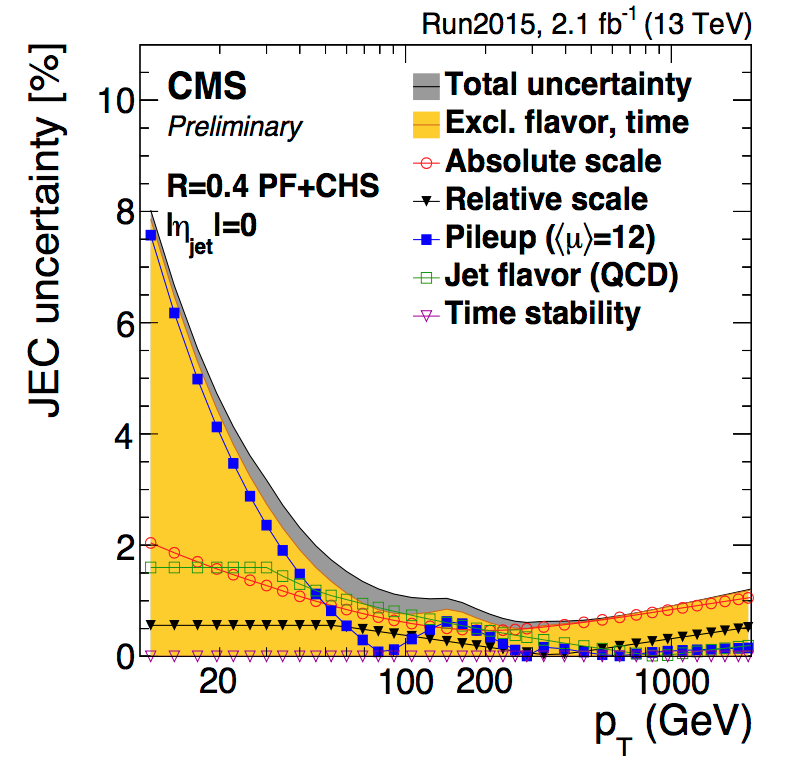
\includegraphics[width=0.8\textwidth]{./Figures/reconstruction/jec_unc.png}
  \caption{\label{fig:jec_unc} The overall uncertainty in the corrections applied to MC from Equation~\ref{equ:jec} shown in the orange solid curve. The pileup uncertainty dominates
for $\pt < 50\GeV$ while for higher values of \pt~the absolute and relative scale dominate~\cite{jec_fig}.}
\end{figure}

\subsection{B tagging}
\label{sec:btag}
For Run 2 the Combined Secondary Vertex version 2 (CSVv2) algorithm is used to tag jets as originating
from b quarks. The algorithm exploits the long lifetime of the b hadron, the secondary vertex of its decay
and the possible presence of a muon or electron (produced in $\sim 20\%$ of the b hadron decays). The 
input variables are combined with a neural net and the secondary vertex
information is obtained using the Inclusive Vertex Finder (IVF) algorithm~\cite{csv_pas}.

The dominant backgrounds for tagging b quarks are jets originating from c quarks and to a lesser extent
jets from lighter quarks and gluons. The distribution of the CSVv2 discriminator is shown for PF Jets
using $13\TeV$~data and simulation in Figure~\ref{fig:csv_fig}. The value of the discriminator
used in the $\alphat$ analysis is 0.89 corresponding to an efficiency of $\sim67\%$ CHECK THIS and 
a mistag rate of $\sim 1\%$ for light quarks ($u$, $d$ and $s$ quarks) and gluons and a mistag rate of $\sim 10\%$ for
charm quarks. The difference in efficiency and mistag rates in data and simulation is measured 
for a range of jet energies to provide scale factors to correct the simulation. In the
Run 2 dataset, these scale factors were around $0.94$ and $\sim1.1-1.3$ (depending on \pt) for the b-tag and mistag SFs 
respectively~\cite{csv_fig}.

\begin{figure}
\centering
    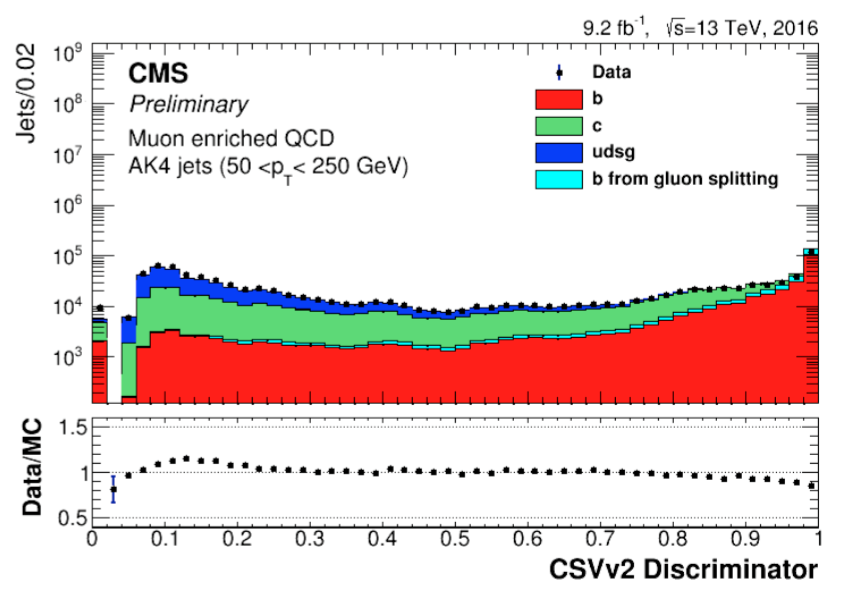
\includegraphics[width=0.8\textwidth]{./Figures/reconstruction/csv_fig.png}
  \caption{\label{fig:csv_fig} Distribution of the CSVv2 discriminator for ak4 jets 
in a muon enriched jet sample (right). The markers correspond to the data. 
The stacked, coloured histograms indicate the contributions of the different 
jet flavours in the simulation~\cite{csv_fig}}
\end{figure}

\subsection{Cross cleaning}

The lepton and jet reconstruction algorithms are run independently and so the same detector
signals may be reconstructed as different physics objects. To avoid this double
counting, a cross cleaning is performed. Any reconstructed jets within $\Delta R < 0.4$ 
of an isolated lepton are removed.

\subsection{Energy sums}
\label{sec:energy_sums_reco}
Energy sums are vital for hadronic searches for new physics such as the $\alphat$~search. The typical high
mass scale of BSM models causes large quantities of energy to be transferred to particles in the final
state. This energy is shared between both visible and invisible particles leading to large total and missing energy
which can be measured by CMS. These signatures provide a crucial separation from the QCD background, typically at
a lower energy scale. The CMS detector is ideally suited to measuring these signatures due to its hermetic design
allowing optimal acceptance for all observable particles in the final state.

To measure the energy scale of the parent process in the event two variables are commonly used. 
These are the total transverse energy, $E_\text{T}$, which is computed as the scalar sum of the transverse 
energies of all reconstructed PF candidates in the event and the total hadronic
transverse energy, \scalht, which is computed as the scalar sum of the transverse energies of all calibrated reconstructed jets:

\begin{equation}
E_\text{T} = \sum |\vec{p}_T^{\text{PF}}| && \scalht = \sum |\vec{p}_\text{T}^{j}|.
\end{equation}

Missing energy in the final state can be caused by BSM phenomena such as the LSP of R-parity conserving SUSY or 
DM particles predicted by generic models of Dark Matter as well as standard
model processes such as neutrinos from vector boson decay. This quantity is reconstructed indirectly from the observed particles in the final state by exploiting
momentum conservation in the transverse plane. Two variables are used in the
\alphat~analysis: the missing transverse momentum, 
\metvec, which is defined as the negative vector sum of the transverse momenta
of all PF candidates and has magnitude \met,
as well as the hadronic missing transverse momentum, \mhtvec, which is defined as the negative vector sum of the
transverse momenta of all calibrated reconstructed jets and has magnitude \mht:

\begin{equation}
\metvec = -\sum \vec{p}_T^{PF} && H_T = -\sum \vec{p}_T^{j}.
\end{equation}

In addition, calorimeter-\metvec, defined as the negative transverse vector sum of the calorimeter deposits, is used 
for the HLT as the PF candidates cannot be reconstructed within latency constraints. The \metvec~is used offline
as the performance is substantially improved by including tracker information~\cite{pf_pas}. 

As a measure of the momentum imbalance, \metvec~can be biased due to effects including 
minimum energy thresholds in the calorimeters, tracker inefficiencies and non=linearities
in calorimeter response. This bias is reduced by correcting the \pt~of CHS corrected PF jets 
using the JECs and propagating the correction to the \metvec~as

\begin{equation}
\vec{E}_\text{T}^{\rm misscorr} = \metvec - \sum_{j}(\vec{p}^{\text{corr},j}_T -
\vec{p}_T^{j}).
\end{equation}

This `type-1' correction~\cite{met_fig}~uses all corrected jets with $\pt > 15\GeV$ with less than 0.9 of their energy deposited in the ECAL.
The 4-momenta of any muons found in jets are subtracted when performing the correction and added back to the corrected object.
Figure~\ref{fig:met_fig} shows excellent agreement between simulation and data
in reconstructing the \met~with 13\TeV~Run 2 data.

\begin{figure}
\centering
    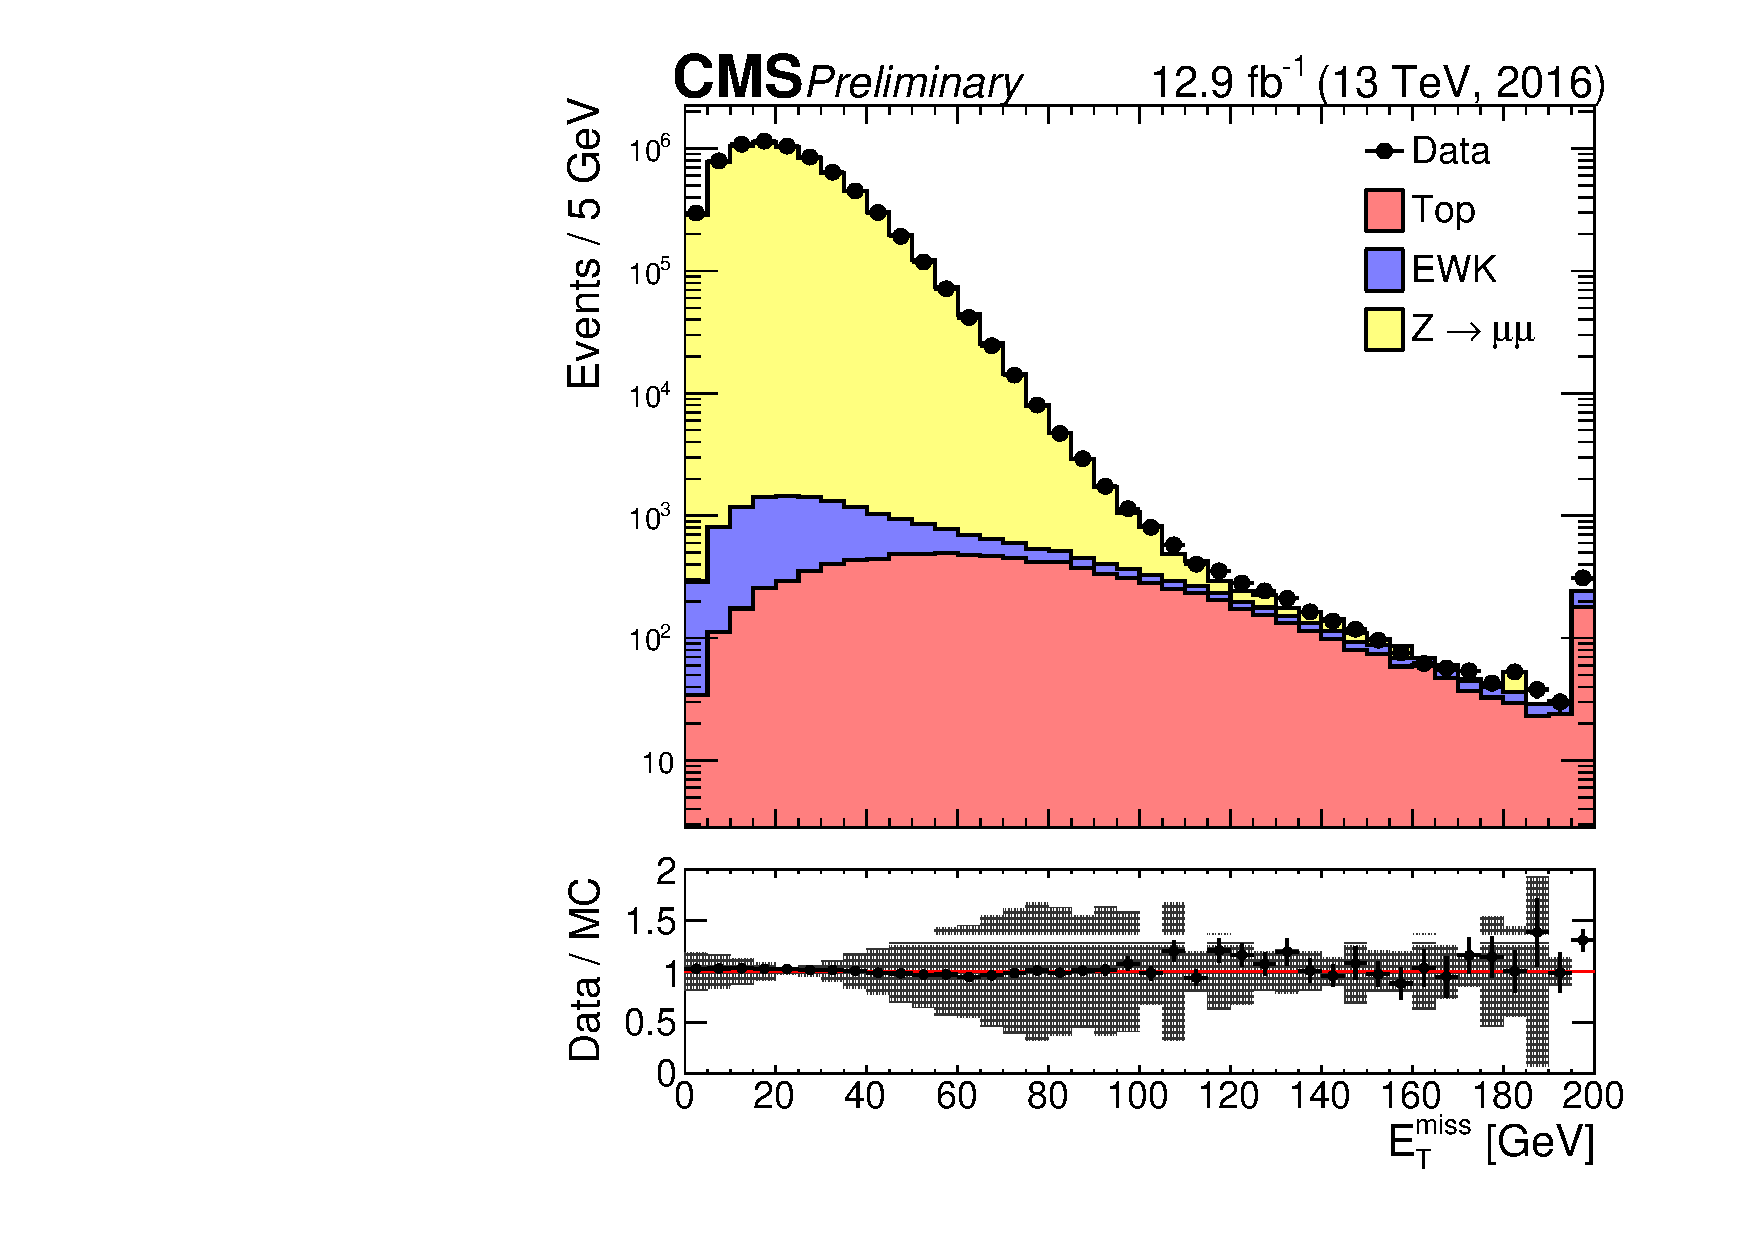
\includegraphics[width=0.8\textwidth]{./Figures/reconstruction/met_fig.pdf}
  \caption{Distribution of \met~in \zmumu candidate events. The markers show the data while the filled coloured histograms
  show the breakdown in difference processes for the simulation. The lower panel shows the data/MC ratio including
  both statistical and systematic uncertainties~\cite{met_fig}. \label{fig:met_fig} 
}
\end{figure}

\section{Physics objects for the \alphat~analysis}

The \alphat~analysis makes use of the reconstruction algorithms described above
to identify and reconstruct physics objects. The analysis uses a hadronic signal 
region with jets and large~\met as well as several signal depleted regions used to predict the
backgrounds in the signal region, the hadronic, \gj, \mj and \mmj control regions defined in 
Section~\ref{sec:cr-sel}. This section describes the definition of the 
physics objects used for the \alphat~analysis.

\label{sec:phys-obj}
\subsection{Jets}

The jet collection is defined by PF jets (clustered from PF candidates) as defined in Section~\ref{sec:jet_reco} with
$\Delta R = 0.4$. The jets are corrected for pileup contributions using CHS and jet area corrections. Additional cleaning cuts are then applied
on the jet constituents as summarised in Table~\ref{tab:loose-jet-id}. These requirements are necessary to reject fake jets. The charged hadron
fraction cut of $> 0.1$ additionally rejects jets reconstructed from beam halo interactions.

A threshold of jet $\pt > 40 \GeV$ is required for jets used in the analysis. As supersymmetric models tend to produce
relatively hard jets this provides a good efficiency while effectively rejecting QCD backgrounds. Jets in the signal 
region must satisfy the pseudorapidity requirement $\etaabs < 2.4$. The presence of any forward jets with $\etaabs > 2.4$
is used as a cleaning veto as described in Section~\ref{sec:fwd_jet_veto}. Additionally, the leading jet in the 
event must satisfy $\pt > 100\GeV$. 
\begin{table}[ht!]
  \caption{Jet identification requirements. \label{tab:loose-jet-id}}
  \centering
  \begin{tabular}{ ccc }
    \hline
    \hline
    Variable & cut & notes \\ \hline
    \multicolumn{3}{c}{$-3.0 < \eta_{\mathrm{jet}} < 3.0$} \\ \hline    
    Neutral Hadron Fraction & $<0.99$ & - \\
    Neutral EM Fraction & $<0.99$ & - \\
    Number of constituents & $>1$ & - \\
    Charged Hadron Fraction & $>0$ & only for $|\eta_{\mathrm{jet}}| < 2.4$ \\
    Charged Multiplicity & $>0$ & only for $|\eta_{\mathrm{jet}}| < 2.4$ \\
    Charged EM Fraction & $<0.99$ & only for $|\eta_{\mathrm{jet}}| < 2.4$ \\ \hline
    \multicolumn{3}{c}{$|\eta_{\mathrm{jet}}| > 3.0$} \\ \hline        
    Neutral EM Fraction & $<0.90$ & - \\
    Number of Neutral Particles & $>10$ & - \\
    \hline
    \hline
  \end{tabular}
\end{table}

\subsubsection{B-tagged jets}

Jets originating from bottom quarks are identified using the CSVv2 algorithm defined in Section~\ref{sec:btag}. 
The tagging efficiency for the working point of the discriminator of 0.89 is $\sim 67\%$ for a mistag rate
of $\sim 1\%$ for light quarks ($u$, $d$ and $s$ quarks) and gluons and a mistag rate of $\sim 10\%$ for
charm quarks.

\subsection{Photons}

Photons must be identified to define the \gj~control region and veto events in the signal and
muon control regions. Their reconstruction is described in Sections~\ref{sec:ele_pho_reco}~and~\ref{sec:particle_flow}. The photon isolation is 
ensured using PF relative isolation with a cone size of $\Delta R = 0.3$. Pileup contributions 
and mitigated using EA correction. Additional selections are summarised 
in Table~\ref{tab:photon-id-gamma} and an efficiency for photon identification of $\sim71\%$
is achieved. The number of fake photons passing selection is measured as $2-10\%$ depending on $\scalht$.

The kinematic selection for photons used to veto events in the signal region is $\pt > 25\GeV$
and $\etaabs < 2.5$. The photons used to define the control region must satisfy the tighter 
requirements $\pt > 25\GeV$ and $\etaabs < 1.4$ to ensure efficient trigger selection and
that the photon is contained within the barrel where it can be better reconstructed.

\begin{table}[ht!]
  \caption{Photon identification requirements.\label{tab:photon-id-gamma}}
  \centering
  \footnotesize
  \begin{tabular}{ ccc }
    \hline
    \hline
    Categories & \multicolumn{2}{c}{Barrel}   \\
    Working point  & Tight & Loose \\
    \hline
    Conversion safe electron veto & Yes & Yes  \\
    Single Tower H/E              & 0.05 & 0.05  \\
    $\sigma_{i\eta i\eta}$        & 0.0100 & 0.0102 \\
    PF charged hadron isolation   & 0.76 & 3.32  \\
    PF neutral hadron isolation   & 0.97 + 0.014 $\times$ $p_{\mathrm{T},\gamma}$ + 0.000019 $\times$ $p_{\mathrm{T},\gamma}^{2}$ & 1.92 + 0.014 $\times$ $p_{\mathrm{T},\gamma}$ + 0.000019 $\times$ $p_{\mathrm{T},\gamma}^{2}$  \\
    PF photon isolation           & 0.08 + 0.0053 $\times$ $p_{\mathrm{T},\gamma}$ & 0.81 + 0.0053 $\times$ $p_{\mathrm{T},\gamma}$ \\
    \hline
    \hline
    Categories & \multicolumn{2}{c}{Endcap}   \\
    Working point  & Tight & Loose \\
    \hline
    Conversion safe electron veto & Yes & Yes  \\
    Single Tower H/E              & 0.05 & 0.05  \\
    $\sigma_{i\eta i\eta}$        & 0.0268 & 0.0274 \\
    PF charged hadron isolation   & 0.56 & 1.97  \\
    PF neutral hadron isolation   & 2.09 + 0.014 $\times$ $p_{\mathrm{T},\gamma}$ + 0.000025 $\times$ $p_{\mathrm{T},\gamma}^{2}$ & 11.86 + 0.014 $\times$ $p_{\mathrm{T},\gamma}$ + 0.000025 $\times$ $p_{\mathrm{T},\gamma}^{2}$ \\
    PF photon isolation           &  0.16 + 0.0034 $\times$ $p_{\mathrm{T},\gamma}$ & 0.83 + 0.0034 $\times$ $p_{\mathrm{T},\gamma}$ \\
    \hline
    \hline
  \end{tabular}
\end{table}

\subsection{Electrons}

Electrons are identified to veto events in the signal and control regions. The full reconstruction is described in
Sections~\ref{sec:ele_pho_reco}~and~\ref{sec:particle_flow}. The isolation uses PF mini-isolation 
with a variable cone size of maximum radius $\Delta R = 0.2$. The requirements are summarised in 
Table~/ref{tab:ele-id}. An overall efficiency for electron selection of $\sim90\%$ is achieved.

The kinematic requirements for electrons used for vetoing are $\pt > 10\GeV$ and $\etaabs < 2.5$.
\begin{table}[h!]
  \caption{Electron identification requirements.\label{tab:ele-id}}
  \centering
  \footnotesize
  \begin{tabular}{ lcc }
    \hline
    \hline
    Categories                                               & Barrel    & EndCap    \\
    \hline
    $\Delta \eta_{In}$                                       & 0.0105   & 0.00814  \\
    $\Delta \phi_{In}$                                       & 0.115    & 0.182  \\
    $\sigma_{i\eta i\eta}$                                   & 0.0103    & 0.0301  \\
    H/E                                                      & 0.104    & 0.0897   \\
    d0 (vtx)                                                 & 0.0261    & 0.118  \\
    dZ (vtx)                                                 & 0.041    & 0.822  \\
    $\lvert(1/E_{\textrm{ECAL}} - 1/p_{\textrm{trk}})\rvert$ & 0.102     & 0.126  \\
    Missing hits (inner tracker)                             & 2         & 1         \\
    Conversion veto                                          & yes       & yes   \\
    \hline
    \hline
  \end{tabular}
  \end{table}
\subsection{Muons}

Muons are selected to define the single mu, $\mj$, and double mu, $\mmj$ control regions as well as 
for veto in defining the signal regions. The reconstruction is described in Section~\ref{sec:muon_reco}.
The isolation is defined using a PF relative isolation requirement of $I_{\text{PF}}^{\text{rel}} < 0.15$ 
with a cone size of $\Delta R = 0.4$ for muons in the control regions and using a PF mini-isolation requirement of
$I_{\text{PF}}^{\text{mini}} < 0.2$ with a maximum cone size of $\Delta R = 0.4$. The muons are pileup corrected
using an EA correction. An efficiency for muon selection of $\sim98\%$ is achieved.

The kinematic requirements for muons used for veto are $\pt > 10\GeV$ and $\etaabs < 2.4$, while muons 
selected in the control regions must satisfy $\pt > 30\GeV$ and $\etaabs < 2.1$. This ensures efficiency
for passing trigger requirements and that the muon is well reconstructed.


\subsection{Isolated tracks}

Isolated tracks are used to identify W boson decays and single prong decays of the $\tau$. 
They are selected from the charged PF candidates satisfying $\pt > 10\GeV$, $\Delta z(\text{track},\text{PV})$ and 
$I_{\text{PF}}^{\text{rel}} < 0.1$ with a cone of $\Delta R = 0.3$.

\subsection{Energy sums}

The $\met$ is computed from the magnitude of the vector sum of the transverse momentum of all PF candidates in
the event. This is type-1 corrected, as described in Section~\ref{sec:energy_sums_reco}, 
using PF jets with $\pt > 15\GeV$. In the control regions the object(s) used to define
the control region is not included the $\met$ calculation. The \mht~and \scalht~are defined
using the vector and scalar sum respectively of all PF jets satisfying $\pt > 40 \GeV$ and $\etaabs < 2.4$.

\subsection{Summary}

A summary of the physics objects used for the \alphat search and their
kinematic requirements is presented in Table~\ref{tab:kine-sel}.

\begin{table}[h!]
  \caption{Kinematic selections for physics objects.\label{tab:kine-sel}}
  \centering
  \footnotesize
  \begin{tabular}{ lll }
    \hline
    \hline
    Object 	& 	&Kinematic selection \\
    \hline
    \hline
    Jet  		&Central jets& $\pt > 40 \GeV,\ \etaabs < 2.4$		    \\
			&Leading central jets&	$\pt > 100 \GeV,\ \etaabs < 2.4$	\\	    	    
			&Forward jet (veto) &$\pt > 40 \GeV,\ \etaabs > 2.4$	\\	    
    Photon  		&\gj control region& $\pt > 200 \GeV,\ \etaabs < 1.45$	\\	    
			&Veto& $\pt > 25 \GeV,\ \etaabs < 2.5$		    \\
    Muon  		&\mj and \mmj control regions& $\pt > 30 \GeV,\ \etaabs < 2.1$	\\	    
			&Veto& $\pt > 10 \GeV,\ \etaabs < 2.5$		    \\
    Electron  		&Veto& $\pt > 10 \GeV,\ \etaabs < 2.5$		    \\
    Isolated track  	&Veto& $\pt > 10 \GeV,\ \etaabs < 2.5$		    \\
		
    
    \hline
    \hline
  \end{tabular}
  \end{table}

% \chapter{Introduction}
\label{cha:introduction}

In the 20th century, great advances have been made in
understanding the properties and interactions of 
the fundamental particles that make up our universe. 
The standard model (SM) of particle physics provides an 
extraordinarily successful description of the phenomena 
that have been observed in a plethora of experiments.

Despite these successes, the SM is known to be incomplete.
From a theoretical perspective, the theory cannot provide a description of gravitational
interactions on a microscopic scale~\cite{gravRenorm}. In addition, multiple astronomical observations 
have supported the existence of a weakly interacting dark matter particle that
comprises around five times more of the mass in the universe than particles 
predicted in the SM~\cite{WIMP}.

Supersymmetry (SUSY) is an additional symmetry between bosonic and fermionic particles 
that is among the best motivated of theories that can resolve these
and other issues of the SM. The features of the SM and SUSY models are detailed 
in Chapter~\ref{cha:theory}. Most supersymmetric theories contain a stable,
weakly interacting lightest supersymmetric particle (LSP) which has the properties 
of a dark matter candidate.

The Large Hadron Collider (LHC) is a proton-proton (p-p) collider designed to probe the 
SM with collisions at the highest ever centre of mass energy (13~\TeV).
The Compact Muon Solenoid (CMS) detector is among two general purpose detectors
designed to provide precise measurements of the energy, position and momenta of
the particles produced in these collisions. The LHC and CMS have run successfully at a lower centre of 
mass energy (7-8~\TeV), discovering the Higgs boson and providing the strongest 
constraints on a range of SUSY models. The LHC and CMS are described in Chapter~\ref{cha:detector}
while the reconstruction of the data collected by CMS is detailed in Chapter~\ref{cha:reco}.

The Level-1 trigger system is a crucial component of the CMS detector, responsible 
for making the initial decision on whether an event should be recorded 
for full analysis. As the data taking conditions become more extreme, the hardware
and algorithms used by this system must be fully upgraded. The jet finding and energy sum algorithms 
are particularly important for SUSY analyses. The Level-1 Trigger upgrade is described in 
Chapter~\ref{cha:triggerUpgrade}. 

The \alphat analysis is a search for SUSY using data recorded by the CMS detector. 
Sensitivity to beyond standard model (BSM) physics requires strong rejection of backgrounds while
maintaining acceptance to signal. Experimental signatures of SUSY include significant
hadronic activity in the form of jets and significant~`missing energy' due to the production
of the LSP. In Chapter~\ref{cha:alphat}, the strategy of the \alphat search is described, which uses
dimensionless variables to mitigate the otherwise dominant background containing fake missing energy.
As shown in Chapter~\ref{cha:alphat}, the \alphat~search achieves inclusive sensitivity 
to a wide range of models by finely categorising events according to 
their energy, missing energy, number of jets and number of b tagged jets.

In order to extract a possible signal contribution, the background components passing selection 
and associated systematic uncertainties must be robustly determined. In Chapter~\ref{cha:backgroundPrediction},
the procedures for determining backgrounds containing true and fake missing
energy are detailed. The systematic uncertainties are determined using tests with 
both data and simulation. 

The compatibility of the data with the SM hypothesis is assessed using a maximum likelihood fit 
as detailed in Chapter~\ref{cha:statisticalResults}. As no evidence is observed for BSM physics,
the results are interpreted using simplified supersymmetric models which evaluate the reach
of the search for different SUSY event topologies. 

Finally, the results of searches cannot be interpreted in the plethora of models to which 
they may be sensitive. A procedure is given to facilitate the re-interpretation
of the \alphat~search, such that its impact on any BSM physics may be approximated.
This procedure is applicable to many searches and is described fully in 
Chapter~\ref{cha:simplifiedLikelihood}.


% \chapter{Theoretical overview}
\label{cha:theory}

In this chapter the current best theory of particle physics, the Standard Model,
is outlined. Outstanding problems are detailed and used to motivate BSM 
physics and, in particular, SUSY. The features of supersymmetric theories are 
outlined and the possible experimental signatures which would enable such a theory to be 
discovered are detailed.

Natural units, Einstein summation convention
and Feynman slash notation are used throughout. Electric charges 
are in units of the charge of the electron.

\section{The Standard Model}

\label{sec:sm}

The SM of particle physics is a quantum field theory (QFT) whose excitations
correspond to the elementary particles forming all known matter and the mediators of
all known forces~\cite{ftsm}. 

The known matter in the universe is composed of spin-1/2 fermions, summarised 
in Table~\ref{tab:fermions}. These are split into quarks which carry colour charge 
(see Section~\ref{sec:sm-gs}) and leptons which do not. In terms of their
quantum numbers, each of the three 
generations of quarks and leptons vary only in mass from the other generations. 
The SM contains spinor fields which give rise to these fermions.

The interactions between particles in the universe are mediated by
spin-1 bosons, summarised in Table~\ref{tab:bosons}. 
The gluon and photon are massless while the W and Z bosons are massive. 
The mechanism for determining the masses of these particles, discussed in 
Section~\ref{sec:sm-gs}, gives rise to a further fundamental spin-0 particle, the Higgs boson.
The SM contains vector and scalar fields which give rise to the spin-1 and spin-0
bosons respectively.

The symmetries of the SM determine the properties of the particles and 
their interactions. There are two classes of symmetries:

\begin{itemize}
\item Space-time symmetries corresponding to translations and rotations of the space-time coordinates.
The SM satisfies the Poincar\'{e} group of space-time transformations that define special relativity. 
\item Gauge symmetries corresponding to transformations of the fields within the SM.
\end{itemize}

The mechanism by which the gauge symmetries give rise to the properties and interactions 
of the particles in the SM is detailed in the remainder of this section. 

\begin{table}
  % \caption[The fundamental spin-1/2 fermions observed in nature separated into their three generations. 
  % Each particle shown also has an antiparticle with opposite charge and identical mass]
  % {The fundamental fermions observed in nature separated into their three generations. 
  % Each particle shown also has an antiparticle with opposite charge and identical mass~\cite{pdg}.}
  \caption[The fundamental spin-1/2 fermions observed in nature separated into their three generations. 
  The u, d and s quark masses are estimates of the `current' quark masses in the $\overline{\text{MS}}$-Scheme at $\mu \sim 2~\GeV$,
  the c and b quark masses are the running masses in the $\overline{\text{MS}}$-Scheme at $\mu \sim2~\GeV$ 
  and all other masses are from direct measurement. Each particle shown also has an antiparticle with opposite charge and identical mass]
  {The fundamental fermions observed in nature separated into their three generations. 
  The u, d and s quark masses are estimates of the `current' quark masses in the $\overline{\text{MS}}$-Scheme at $\mu \sim 2~\GeV$,
  the c and b quark masses are the running masses in the $\overline{\text{MS}}$-Scheme at $\mu \sim2~\GeV$ 
  and all other masses are from direct measurement. Each particle shown also has an antiparticle with opposite charge and identical mass~\cite{pdg}.}
  \label{tab:fermions}
  \begin{tabular}{ccccccc}
  \hline\hline
  &\multicolumn{3}{|c|}{Leptons}& \multicolumn{3}{c}{Quarks} \\
  \cline{2-7}
  Generation & \multicolumn{1}{|c}{Particle} & Mass & \multicolumn{1}{c|}{Electric Charge} & Particle & Mass & Electric Charge \\
  \hline
  \multirow{2}{*}{1} & \Pem & 511 \keV & -1 & \Pqu & 2.3 \MeV & $+\frac{2}{3}$ \\
  & \Pgne & $\sim$0 & 0 & \Pqd & 4.8 \MeV & $-\frac{1}{3}$ \\
  \hline
  \multirow{2}{*}{2} & \Pgmm & 105.7 \MeV & -1 & \Pqc & 1.275 \GeV & $+\frac{2}{3}$ \\
  & \Pgngm & $\sim$0 & 0 & \Pqs & 95 \MeV & $-\frac{1}{3}$ \\
  \hline
  \multirow{3}{*}{2} & \Pgtm & 1.777 \GeV & -1 & \Pqt & 173.2 \GeV & $+\frac{2}{3}$ \\
  & \Pgngt & $\sim$0 & 0 & \Pqb & 4.18 \GeV & $-\frac{1}{3}$ \\
  \end{tabular}
\end{table}

\begin{table}
  \caption[The fundamental spin-1 vector bosons observed in nature and the force which they mediate.
  Masses are from direct measurement.]{The fundamental spin-1 vector 
bosons observed in nature and the force which they mediate. Masses are from direct measurement~\cite{pdg}.}
  \label{tab:bosons}
  \begin{tabular}{lccc}
    \hline\hline
    Force & Particle & Mass & Electric Charge \\
    \hline
    Electromagnetism & \Pgg & 0 & 0 \\
    \hline
    \multirow{2}{*}{Weak} & \PWpm & 80.4 \GeV & $\pm 1$ \\
    \cline{2-4}
    & \PZ & 91.2 \GeV & 0 \\
    \hline
    Strong & g & 0 & 0 \\
  \end{tabular}
\end{table}

\subsection{Gauge symmetries}

The derivation in this section follows that in Reference~\cite{ewk-int}. Consider a Lagrangian containing a fermionic field, $\psi$,

\begin{equation}
\mathcal{L} = \bar{\psi}(x) (i\gamma^{\mu}D_{\mu} - m)\psi(x) = \bar{\psi}(x) (i\cancel{D} - m)\psi(x),
\end{equation}

\noindent where $\bar{\psi}(x)$ is the Dirac conjugate of $\psi(x)$, $D_{\mu}$ is the `covariant derivative' and
$\gamma^{\mu}$ are the Dirac matrices. Consider a local gauge symmetry defined by symmetry operator $U(x)$ such that

\begin{align}
\psi(x) &\rightarrow U(x)\psi(x), \\
\bar{\psi}(x) &\rightarrow \bar{\psi} (x) U^{\dagger} (x),
\end{align}

\noindent where $U^{\dagger}(x)$ is the hermitian conjugate of $U(x)$. In the remainder of this section the dependence on $x$ is implicit. In order to ensure gauge invariance, the 
covariant derivative must transform as 

\begin{equation}
\label{equ:cov_deriv}
D_{\mu}\psi \rightarrow U D_{\mu}U^{\dagger} U \psi \rightarrow U \psi.
\end{equation}

\noindent This may be achieved by introducing a vector gauge field, $A_\mu$, such that 
$D_{\mu} = \partial_{\mu} + igA_{\mu}$. To satisfy Equation~\ref{equ:cov_deriv},
such that the Lagrangian is gauge invariant, $A_{\mu}$ must transform
under the `adjoint action',

\begin{equation}
A_{\mu} \rightarrow U A_{\mu} U^{\dagger} + \frac{i}{g}(\partial_{\mu}U)U^{\dagger}.
\end{equation}

\noindent Having introduced this vector field, a new gauge invariant term may be added to the Lagrangian,

\begin{equation}
\mathcal{L} = \bar{\psi} (i\cancel{D} - m)\psi - \frac{1}{4}F^{\mu\nu}F_{\mu\nu},
\end{equation}

\noindent where $F^{\mu\nu}$ is the field strength tensor of the vector field,

\begin{equation}
F_{\mu\nu} = - \frac{1}{g}\left[D_{\mu},D_{\nu}\right] = \partial_{\mu}A_{\nu} - \partial_{\nu} A_{\mu} - g\left[A_{\mu},A_{\nu}\right].
\end{equation}

\noindent By writing the fields and covariant derivatives in terms of the generators of the group, $t_{a}$, such
that $A_{\mu} = A^{a}_{\mu} t_{a}$, the field strength tensor can be written as 
\begin{equation}
F^{a}_{\mu\nu}t_{a} = \left(\partial_{\mu}A^{a}_{\nu} - \partial_{\nu} A^{a}_{\mu} - g f_{bc}^{a}A^b_{\mu}A^c_{\nu}\right)t_a,
\end{equation}
where $f_{bc}^{a}$ are the structure constants of the group defined by the 
commutation of the group generators~\cite{wei1963lie}. Non zero structure constants introduce
self interactions of the gauge fields. No gauge invariant term quadratic 
in $A^a_\mu$ (mass term) can be added to the Lagrangian and 
therefore the vector field is massless.

Gauge symmetries of the Lagrangian therefore result in massless vector 
bosons that are `mediators' of the resultant forces. The properties of
the forces depend on the details of the gauge symmetry. 
In the next section, the gauge symmetries
of the SM are discussed. 

\subsection{Gauge symmetries of the Standard Model}
\label{sec:sm-gs}
The gauge symmetry group of the SM is given by~\cite{ewk-int}:
\begin{equation}
G_{SM} = SU(3)_{c}\otimes SU(2)_{L}\otimes U(1)_{Y}.
\end{equation}

The $SU(3)_c$ gauge symmetry is unbroken and therefore the associated
`strong force' is mediated by a massless vector boson, the gluon.
$SU(3)_c$ is generated by the eight Gell-Mann matrices which give rise to eight colour charges. 
The quarks carry a single colour charge, the gluon is doubly charged and all 
other fundamental particles in the SM are colour singlets. The strong force is short range
as the gluon is self-interacting.  The strong coupling constant, $\alpha_s$, 
reduces with energy (asymptotic freedom)
making calculations non-perturbative~\cite{qcd}. The energy required to separate 
colour singlets of quarks is sufficient to generate additional quark/antiquark pairs
(hadronisation) and therefore quarks are `confined' into colour singlet hadrons
of two (mesons) or three (baryons) quarks. High energy collisions of protons, 
such as those at the LHC, result in the production of highly 
collimated emissions of hadrons (jets) due to the 
liberation of quarks~\cite{salam}.


The gauge symmetry of the electroweak sector of the SM is $SU(2)_L\otimes U(1)_Y$. These symmetries lead
to the electromagnetic and weak forces mediated by the $\gamma$ and W/Z and bosons respectively.
The Lagrangian for this sector may be written as

\begin{equation}
\mathcal{L}_{Ewk} = \mathcal{L}_{gauge} + \mathcal{L}_{fermion} + \mathcal{L}_{Higgs} + \mathcal{L}_{Yuk},
\end{equation}

\noindent the terms of which are discussed in this section. The weak force distinguishes
between left and right-handed chiralities and therefore the fermionic fields are split into
$\psi_{L/R} = (1\pm\gamma^5)\psi$. The fermion term may then be written for each of the 
three generations of quarks and leptons as:

\begin{equation}
\mathcal{L}_{fermion} = i \psiLb\cancel{D}\psiL + i \psiRb\cancel{D}\psiR.
\end{equation}

\noindent The left-handed fields transform as doublets under the $SU(2)_L$ symmetry
while the right-handed fields are singlets.
For the first generations of quarks and leptons $\psi$ may therefore be written as

\begin{align}
\qquad\qquad\qquad\psiL =\,&{\begin{pmatrix} u_L \\ d_L \end{pmatrix}},\, &{\begin{pmatrix} \nu_{e\,L} \\ e_L \end{pmatrix}},\nonumber\qquad\qquad\qquad\\
\qquad\qquad\qquad\psiR = \,&\,u_R,d_R,\, &\,e_R.\qquad\qquad\qquad
\end{align}

\noindent The generators of $SU(2)_L$ are $T^i = \tau^i/2$, where $\tau^i$ are the three Pauli matrices. 
The covariant derivative therefore acts on the left and right-handed components of $\psi$ as

\begin{equation}
D_{\mu} \psiL = (\partial_\mu + igW^i_{\mu}T^i + ig'YB_\mu)\psiL \quad D_{\mu} \psiR = (\partial_\mu + ig'YB_\mu)\psiR
\end{equation}

\noindent where $g$ and $g'$ are the coupling constants of the $SU(2)_L$ and $U(1)_Y$ groups respectively, 
$W^i$ are the three gauge bosons that couple to the weak isospin, $T$, and $B$ is the gauge boson
coupling to hypercharge, $Y$. The hypercharge values are chosen such that the sum of the hypercharge and 
the third component of weak isospin corresponds to the electric charge,
\begin{equation}
\label{equ:charge}
Q = T^{3} + Y.
\end{equation}

\noindent For the gauge section of the Lagrangian, the $SU(2)_L$ and U(1) symmetries give rise to two field strength tensors,
\begin{align}
G^i_{\mu\nu} &= \partial_\mu W^i_\nu - \partial_\nu W^i_\mu - g \epsilon^{ijk}W^j_\mu W^k_\nu,\\
F_{\mu\nu} &= \partial_\mu B_\nu - \partial_\nu B_\mu.
\end{align}

\noindent This leads to

\begin{equation}
\mathcal{L}_{gauge} = -\frac{1}{4}F^{\mu\nu}F_{\mu\nu} - \frac{1}{4}G^{i\mu\nu}G^{i}_{\mu\nu}.
\end{equation}

\noindent The Lagrangian invariant under these gauge symmetries, however, does not correspond to the observed universe. No mass terms
can be included for either the gauge bosons or the fermions while maintaining gauge invariance.
As shown in the remainder of this section, such masses must be introduced via the breaking
of the electroweak gauge symmetry in the Higgs sector of the Lagrangian. This 
sector of the Lagrangian is given by

\begin{equation}
\label{equ:higgs-lagrangian}
\mathcal{L}_{Higgs} = (D^{\mu}\phi)^{\dagger}(D_{\mu}\phi) - V(\phi),
\end{equation}

\noindent where the complex scalar field, $\phi$, is an $SU(2)_L$ doublet. The covariant derivative of $\phi$ is

\begin{equation}
D_{\mu} \phi = (\partial_\mu + igW^i_{\mu}T^i + ig'\frac{1}{2}B_\mu)\phi 
\end{equation}

\noindent and the potential, V, is given by

\begin{equation}
V(\phi) =  - \mu^2\phi^{\dagger}\phi + \lambda \left(\phi^{\dagger}\phi\right)^2,
\end{equation}

\noindent where $\mu^2$ and $\lambda$ are positive constants. The potential is minimised for any $\phi$ satisfying
$\phi^{\dagger}\phi = \frac{\mu^2}{2\lambda} \equiv v^2/2$. While the potential satisfies the 
electroweak gauge symmetry, the minimum will not and may be chosen as

\begin{equation}
\braket{\phi} =  - \frac{1}{\sqrt{2}}\begin{pmatrix} 0 \\ v\end{pmatrix}.
\end{equation}

\noindent From Equation~\ref{equ:charge}, the scalar field has zero electric charge and electromagnetism
is an unbroken symmetry. The symmetry group has therefore been broken 
from $SU(2)_L\otimes U(1)_Y \rightarrow U(1)_Q$. Taking the unitary gauge to remove unphysical `Goldstone 
bosons', the scalar field may be expanded around this minimum as

\begin{equation}
\label{equ:phiExp}
\phi =  - \frac{1}{\sqrt{2}}\begin{pmatrix} 0 \\ v + H\end{pmatrix}.
\end{equation}

\noindent The physical W, Z and $\gamma$ (labelled A) gauge bosons are combinations of the 
bosons defined above,

\begin{equation}
W^{\pm} = \frac{1}{\sqrt{2}} (W^1_\mu \mp i W^2_\mu), \begin{pmatrix} Z_\mu \\ A_\mu\end{pmatrix} = \begin{pmatrix} \cos(\theta_W) & -\sin(\theta_W) \\ \sin(\theta_W) & \cos(\theta_W)\end{pmatrix} \begin{pmatrix} W^3_\mu \\ B_\mu\end{pmatrix}
\end{equation}

\noindent where $\theta_W \equiv \text{atan}(g'/g)$ is the weak mixing angle. From Equation~\ref{equ:phiExp} and
the first term of Equation~\ref{equ:higgs-lagrangian}, the masses may be identified as

\begin{equation}
M_W^\pm = \frac{1}{2}gv, M_Z = \frac{gv}{2\cos\theta_W}, M_A = 0
\end{equation}

\noindent The masses of the fermions are derived from the Yukawa term in the Lagrangian, 
\begin{equation}
\mathcal{L}_{Yuk} = - \frac{1}{\sqrt(2)}(v + H)(f_{mn} \bar{e}_{Lm}e_{Rn} + h_{mn} \bar{d}_{Lm}d_{Rn} + k_{mn} \bar{u}_{Lm}u_{Rn}) + \text{hermitian conjugate}
\end{equation}

\noindent where $f_{mn}$, $h_{mn}$ and $k_{mn}$ are the Yukawa coupling matrices between the different generations. These may be diagonalised via unitary transformations
to generate mass terms for the quarks and leptons. The neutrino is massless in the SM as there is no right-handed component.
This contradicts the observation of oscillations between neutrino flavours~\cite{neutOsc};
however, extensions which predict non-zero neutrino masses are possible~\cite{neutM}. 

The same unitary transformations also introduce mixing between quark generations from the 
terms including covariant derivatives in the Lagrangian. The mixings are summarised in the 
CKM matrix and occur as no basis of mass eigenstates is simultaneously diagonal for 
up and down type quarks~\cite{CKM}. Flavour changing
interactions between quarks are mediated by the $W^{\pm}$ boson while interactions via 
the Z and $\gamma$ bosons are flavour preserving. There are no flavour changing interactions
predicted for the leptons.

\section{Physics beyond the Standard Model}

The SM describes the properties and interactions between all known particles. These properties 
have been measured and the predictions of the SM verified in a multitude
of experiments. However, the theory cannot be complete 
as there remain fundamental problems which the SM does not resolve.
Several of the largest such problems are described below.

On a theoretical level, a renormalisable theory of gravity cannot be included within 
the SM~\cite{gravRenorm}. While negligible at electroweak energy
scales, quantum gravitational effects become increasingly important as
energies approach the planck scale, $M_{\text{planck}} \sim 10^{18} \GeV$. 

Measurements from cosmology and astrophysics have highlighted several areas
the SM fails to adequately describe Nature. The vacuum energy density 
of the universe (`cosmological constant'), $\Lambda$, 
may be expected to be approximated by $M^4_{\text{planck}}$ by dimensional 
arguments. However, cosmological measurements of $\Lambda$ imply 
$\Lambda/M_{\text{planck}}^4 \sim 10^{-120}$~\cite{cosConst}. This discrepancy
is related to the failure to include gravity in a quantum field theory.

Astronomical observation imply the existence of a DM particle
that forms the majority of the matter within the universe
and that does not interact through the strong or electromagnetic forces~\cite{WIMP}.
The SM has no viable candidate for this particle. In addition, the matter-antimatter 
asymmetry observed in the universe requires 
charge-parity violating processes far in excess of those occurring in the SM.

The discovery of the Higgs boson at $m_{h}\sim125\,\GeV$ raises the `hierarchy problem'. 
In QFT, the corrections to $m_h$ are related to the highest energy scale in the theory.
Assuming that quantum effects of gravity are non-negligible at the planck scale 
one may expect $m_h \sim M_{\text{planck}}$ (see Section~\ref{sec:natSUSY}), differing
from the observed mass by many orders of magnitude.

These problems form the motivation for the existence of a BSM physics model that
can resolve some or all of the outstanding issues in the SM. SUSY is a particularly
well motivated BSM theory that can resolve the hierarchy problem, provide a DM candidate
and include a quantum theory of gravity.

\section{Supersymmetry}

There are many possibilities for extending the SM, 
including new particles/interactions, new (internal) gauge symmetries, 
extra spatial dimensions and/or new space-time (external) symmetries. SUSY is 
an external symmetry that relates fermions and bosons by extending the Poincar\'{e} algebra~\cite{SUSYP}. 
The Coleman-Mandula theorem shows that any such extension through new bosonic generators (such as those responsible for Lorentz 
transformations and translations) forbids non-zero scattering amplitudes~\cite{Coleman}. 
Supersymmetry therefore introduces fermionic generators, Q, such that (heuristically),

\begin{equation}
Q\ket{\text{Boson}} \sim \ket{\text{Fermion}} \quad Q\ket{\text{Fermion}} \sim \ket{\text{Boson}}.
\end{equation}

Particles connected by the SUSY generator are in `supermultiplets'. This generator commutes with all gauge symmetries 
of the SM and so particles within each supermultiplet have identical electric, weak isospin and colour charges.
In addition, the SUSY generator commutes with the mass operator, implying 
particles within each supermultiplet have identical masses. The supersymmetric partners of the 
known SM particles, `sparticles', have not been observed and therefore SUSY must be a broken symmetry.

\subsection{The minimally supersymmetric standard model}

The minimally supersymmetric standard model (MSSM) is the simplest supersymmetric extension of the SM~\cite{SUSYP}.
The fermions in the SM are `chiral' (left and right-handed pieces transform differently)
with two fermionic degrees of freedom per helicity state. The number of bosonic and fermionic degrees 
of freedom must be equivalent in each supermultiplet and therefore the simplest supermultiplet
is the chiral supermultiplet containing the fermion and two real scalar fields.

The gauge bosons in the SM (before electroweak SUSY breaking) are massless spin-1 vector bosons
and therefore have two bosonic degrees of freedom (one per helicity state) and
can be included in a `gauge' supermultiplet with a spin-1/2 fermionic partner (`gaugino').

The SM Higgs does not reside in a single chiral supermultiplet as this introduces
a gauge anomaly into the theory~\cite{SUSYP}. This anomaly may be avoided by including two Higgs 
chiral supermultiplets with opposite hypercharge. The SM Higgs is a linear combination of the neutral components 
of these supermultiplets.

\begin{table}[!h]
  \centering
  \caption{Chiral supermultiplets in the MSSM~\cite{SUSYP}}
  \label{tab:chiral}
  \begin{tabular}
    {ccc}
    \hline\hline
    Name& spin-0 & spin-1/2 \\
    \hline
    \multirow{3}{*}{squarks, quarks (3 families) }& ($\tilde{u}_L\,\tilde{d}_L$) & ($u_L\,d_L$) \\
    & ($\tilde{u}^{*}_R$) & ($u_R^{\dagger}$) \\
    & ($\tilde{d}^{*}_R$) & ($d_R^{\dagger}$) \\
    \hline
    \multirow{2}{*}{sleptons, leptons (3 families) }& ($\tilde{\nu}\,\tilde{e}_L$) & ($\nu_L\,e_L$) \\
    & ($\tilde{e}^{*}_R$) & ($e_R^{\dagger}$) \\
    \hline
    \multirow{2}{*}{Higgs, higgsinos}& ($H_u^{+}\,H_u^{0}$) &  ($\tilde{H}_u^{+}\,\tilde{H}_u^{0}$) \\
    & ($H_d^{0}\,H_d^{-}$) &  ($\tilde{H}_d^{0}\,\tilde{H}_d^{-}$) \\
  \end{tabular}
\end{table}

\begin{table}[!h]
  \centering
  \caption{Gauge supermultiplets in the MSSM~\cite{SUSYP}}
  \label{tab:vector}
  \begin{tabular}
    {ccc}
    \hline\hline
    Name& spin-1/2 & spin-1 \\
    \hline
    gluino, gluon & $\tilde{g}$ & g \\
    winos, W bosons & $\tilde{W}^{\pm}\,\tilde{W}^0$ & $W^{\pm}\,W^{0}$ \\
    bino, B boson & $\tilde{B}^0$ & B \\
  \end{tabular}
\end{table}

The particle content of the MSSM (before symmetry breaking) 
is summarised in Table~\ref{tab:chiral} for the chiral supermultiplets
and Table~\ref{tab:vector} for the gauge supermultiplets. The neutral higgs and electroweak 
gaugino sectors combine to form mass eigenstates labelled `neutralinos' 
(\chiz), while the charged higgs and electroweak gaugino sectors combine
to form `charginos' (\chip). Gravity may also be included in the theory
by adding a spin-2 graviton and a spin-3/2 superparticle
called the gravitino~\cite{SUSYP}. 

The mass scale of the sparticles is dependent on the mechanism of SUSY breaking.
As discussed below, naturalness arguments motivate the lightest sparticle masses 
at the \TeV~scale.

\subsection{Natural supersymmetry}
\label{sec:natSUSY}
In the SM, the Higgs mechanism requires couplings to each fermion, $f$, of the form $-\lambda_{f}\bar{f}\phi f$. If BSM physics
is expected to alter the high energy behaviour of the theory at a scale $\LUV$, the quantum corrections 
to the Higgs boson mass, $\delta m^2_{H}$, will be 

\begin{equation}
\Delta m^2_H =  \frac{|\lambda_f|^2}{8\pi^2}\left[-\Lambda^2_{\text{UV}}\right] + \mathcal{O}\left(\log(\LUV)\right)
\end{equation}

\noindent which is quadratically divergent~\cite{SUSYP}. The correction is proportional to the size of the coupling of the Higgs to the fermion 
and is therefore largest for the top quark in the SM. Assuming the cut-off scale is at $M_{\text{planck}}$, the quantum 
corrections must be fine-tuned to $\sim 30$ orders of magnitude to predict the observed Higgs mass. 

In a BSM theory containing complex scalars, $s$, the Lagrangian will gain a term $-\lambda_{s}|\phi|^2|s|^2$.
Assuming, for simplicity, each component of the complex scalar has mass $m_s$, the correction to the Higgs mass will be

\begin{equation}
\label{equ:corrHiggsSusy}
\Delta m^2_H =  \frac{\lambda_s}{8\pi^2}\left[-\Lambda^2_{\text{UV}}\right] + \mathcal{O}\log(\LUV).
\end{equation}

If SUSY is a symmetry of nature, each fermion can be related to a complex scalar such that $|\lambda_f|^2 = -\lambda_s$ 
and the quadratic divergence is naturally cancelled. In unbroken SUSY, logarithmic divergences also vanish~\cite{SUSYP}. 
Experimental observations imply the sparticle masses cannot be equal to their SM partners and
therefore an additional SUSY breaking term is required in the Lagrangian. This must be a `soft' breaking,
such that $\lambda_f^2 = -\lambda_s$ still holds to cancel the quadratic divergence.
To avoid fine tuning of the logarithmic divergence, the lightest sparticles should have 
masses around the $\TeV$ scale. The LHC provides the first experimental probe of this energy scale.

While such arguments provide a strong motivation for $\TeV$ scale gluinos and squarks, it
should also be noted that models such as 'split SUSY`~\cite{sSusy} or the 'AMSB`~\cite{AMSB} provide alternative
solutions to the naturalness problem with significantly different signatures at the LHC (see below).

\subsection{R-parity}

The general MSSM `super potential' contains terms which violate baryon number, B, and lepton number, 
L. Such terms lead to predictions of proton decay in the order of seconds. 
The proton lifetime is constrained experimentally to $> 10^{34}$ years~\cite{protonDecay};
therefore, to forbid such a process, an extra symmetry called `R-parity' is defined as,
\begin{equation}
R \equiv (-1)^{3(B-L)+2S} = 
\begin{cases}
+ 1\quad \text{SM particles}\\
- 1\quad \text{superpartners}
\end{cases},
\end{equation}
where S is the spin~\cite{SUSYP}. R-parity has several physical implications including a stable lightest supersymmetric 
particle (LSP). This particle must be electrically and colour-neutral from cosmological constraints.
Typically, it is taken to be the lightest neutralino in the MSSM.
This LSP is a weakly interacting massive particle (WIMP) and is candidate for DM. 
In addition, R-parity requires that superpartners be
formed in pairs in collisions and that each superpartner decays to another superpartner
in a chain that must end with the LSP. The interactions of the LSP with detectors at the LHC
are too weak to be observed and therefore such collisions will produce signatures 
containing significant momentum imbalance.

\subsection{Experimental SUSY signatures at the LHC}

The LHC provides proton-proton collisions at $\sqrt{s} = 13\,\TeV$. The sparticles have identical charges under 
the symmetries of the SM and, therefore, in a generic (natural) MSSM model 
coloured sparticles may be expected to have the highest production 
cross-section~\cite{susyprod}. Assuming R-parity, these sparticles can be produced through:

\begin{itemize}
\item quark-antiquark scattering or gluon fusion to produce a gluino or squark pair
\item quark and gluon scattering to produce a squark and gluino
\item quark-quark scattering to produce a squark pair.
\end{itemize}

Each of the sparticles will decay in a chain to the LSP. In the decay, 
coloured SM particles are produced which will hadronise into jets.
The signature produced by such processes will therefore be significant hadronic activity in 
the form of jets as well as momentum imbalance from the LSP. The energy in
the final state and the momentum carried by the LSP are dependent on the masses
of the sparticles.

The top makes the largest contribution to the Higgs boson mass divergence. In natural SUSY, 
the lightest coloured sparticle is expected, therefore, to be the partner of the top. This leads to a signature
of multiple top quarks in the final state. As discussed in Section~\ref{sec:ewk-background-intro}, top quarks
decay primarily to a b quark and W boson. The sparticles produced at the LHC 
may therefore be expected to lead to a final state containing multiple b quarks.

The SM contains processes which produces events with similar signatures to 
those of hadronic SUSY described above. These are described fully in Section~\ref{sec:ewk-background-intro},
and, in order to be sensitive to SUSY signals, such background processes must be mitigated 
and any residual background contributions measured. The search described in this thesis relies on several
techniques to mitigate and measure background processes as described in Chapters~\ref{cha:alphat} and~\ref{cha:backgroundPrediction},
respectively.

\subsection{Simplified models}

The MSSM contains up to 120 free parameters that affect the production and decay modes of the sparticles.
It is therefore not possible to interpret the results of searches for SUSY in the full MSSM. 
In previous searches for SUSY, the constrained MSSM (the CMSSM), which leaves five free parameters, was 
used to interpret the results~\cite{CMSSM}. However, while parametrically simple, the decay chains of sparticles 
in the CMSSM are complicated, making such interpretations model-dependent. 

To evaluate model-independent reach, searches are interpreted using 
simplified models that are defined by a fixed set of production and decay modes.
Simplified models are effective models where the majority of the particle content in the theory 
is decoupled at high masses. Each of the simplified models considered in this thesis involves
the direct pair production of only one sparticle type, which then decays directly to the LSP~\cite{SMS}.

The simplified models may be used to approximate the impact of searches on a complete theory 
by determining the relevant simplified topologies contained in the full theory. The impact
of searches for many different types of signatures may be combined using programs 
such as FastLim~\cite{Fastlim}.

The T2 simplified models are simplified versions of squark-antisquark production. Each squark undergoes
a two-body decay to a quark and the LSP. In this thesis, direct bottom squark production followed
by decay to bottom quark and LSP as well as direct top squark production followed by decay to top
quark and LSP are considered.

The T1 simplified models are simplified versions of gluino pair production. Each gluino undergoes a three-body 
decay to a quark-antiquark pair and the LSP. In this thesis, decays to top-antitop as well as bottom-antibottom
pairs are considered. As the three body decay proceeds via the virtual squark, these models 
are referred to as gluino-mediated squark production.

\begin{figure}[h!]
  \begin{center}
    \subfloat[Gluino mediated bottom squark production]{
      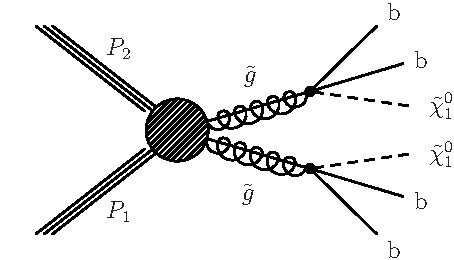
\includegraphics[width=0.4\textwidth]{Figures/theory/T1bbbb_feyn}
      \label{fig:T1bbbb_feyn}
    } ~~
    \subfloat[Glunio mediated top squark production]{
      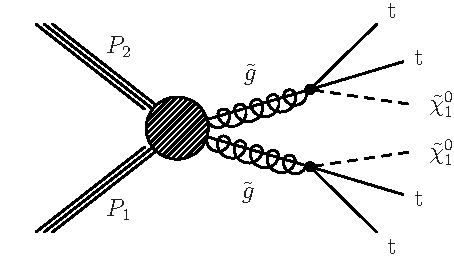
\includegraphics[width=0.4\textwidth]{Figures/theory/T1tttt_feyn}
      \label{fig:T1tttt_feyn}
    } \\
    \subfloat[Direct bottom squark production]{
      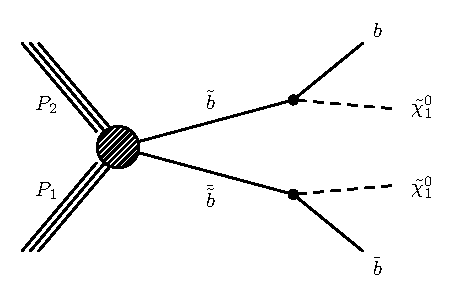
\includegraphics[width=0.4\textwidth]{Figures/theory/T2bb_feyn}
      \label{fig:T2bb_feyn}
    } ~~
    \subfloat[Direct top squark production]{
      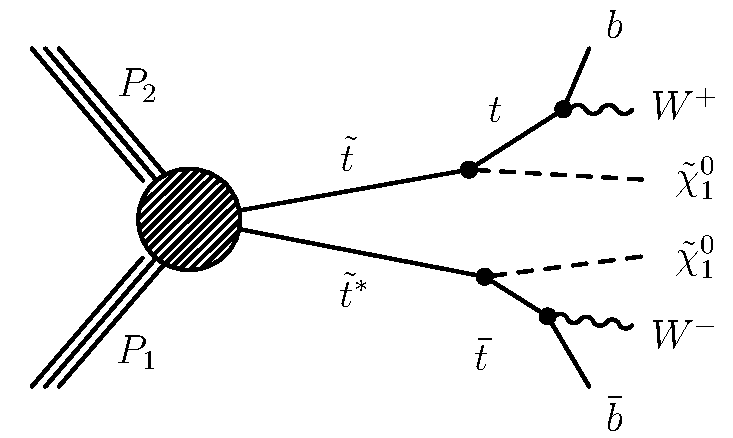
\includegraphics[width=0.4\textwidth]{Figures/theory/T2tt_feyn}
      \label{fig:T2tt_feyn}
    } 
    \caption{
      Graphical representation of the production and decay of supersymmetric particles 
      for the simplified models considered in this thesis~\cite{SMS}.
    }
    \label{fig:simplified-models-feyn}
  \end{center}
\end{figure}

Figure~\ref{fig:simplified-models-feyn} displays the decay chains for the models considered in this thesis. 
In the simplified models, the masses of the heavy sparticle and of the LSP are free parameters.
The topology of the model is crucial in determining the reach of experimental searches. 
In cases where the mass splitting is large, the final state typically contains significant
momentum imbalance and hadronic energy. If the mass splitting is small, (`compressed' models),
the momentum imbalance and hadronic energy are suppressed. Additional phenomena, such as initial/final state radiation (ISR/FSR), 
where one or more incoming/outgoing partons radiates a jet, may be required for sensitivity to such models.

The furthest mass points excluded (see Section~\ref{sec:limits}) by searches at CMS for a 
range of simplified supersymmetric models at the end of the 7 and 8~\TeV~centre of mass 
energy runs of the LHC are shown in Figure~\ref{fig:CMS2014}. The searches carried out target a range 
of natural SUSY scenarios. The hadronic searches require a final state containing 
no leptons or photons and are sensitive to SUSY models containing light squarks and gluinos. Searches for electroweak
gauginos use a wide variety of final states containing vector bosons (or their decay products) 
to achieve sensitivity to SUSY models with light charginos and neutralinos~\cite{gaugino}. 
The discovery of the Higgs boson has motivated additional searches for 
neutralino decay to the Higgs boson and LSP, sensitive to models
with higgsino neutralinos and charginos~\cite{gmsb}. The search for the SUSY partner of the lepton is sensitive 
to models which can provide the muon anomalous magnetic moment from SM expectation~\cite{gm2}. Finally,
there are searches for SUSY models in which R-parity is not conserved (RPV SUSY) that 
typically require a large number of jets and low~\met~\cite{rpv}. In addition to such 'prompt` analyses, 
searches for long lived particles (not shown in Figure~\ref{fig:CMS2014}), 
can be sensitive to SUSY models with very small mass splittings~\cite{llpSUSY}. A full review of 
all signatures and searches at both CMS and ATLAS may be found in Reference~\cite{pdg}.

\begin{figure}
\centering
    \includegraphics[width=0.9\textwidth]{./Figures/theory/barplot_ICHEP2014}
  \caption{
  Best exclusion limits for the masses of the parent particles for
  $m_{\text{LSP}} = 0 \,\GeV$ (dark shades) and $m_{\text{parent}} - m_{\text{LSP}} = 200\,\GeV$ 
  (light shades); for each topology, for all results~\cite{susyCMS2014}.
  }
  \label{fig:CMS2014}
\end{figure}

As the centre of mass energy increases to $13\,\TeV$, searches for a wide
range of signatures, including those detailed above, are necessary to 
explore potential SUSY models. Hadronic searches, such as the \alphat analysis, 
present a particularly exciting opportunity as the production 
cross-section for for coloured sparticles at the~\TeV~scale 
jumps by more than an order of magnitude~\cite{snowmass}.

\end{mainmatter}

% \bibliographystyle{unsrt}
% \bibliography{thesis}
% %\printbibliography

% Produce the appendices
\begin{appendices}
  \chapter{Appendix}
\label{app:test}
lorem ipsum


\end{appendices}

% Produce the un-numbered back matter (e.g. colophon,
% bibliography, tables of figures etc., index...)
\begin{backmatter}
 
%% You're recommended to use the eprint-aware biblio styles which
%% can be obtained from e.g. www.arxiv.org. The file mythesis.bib
%% is derived from the source using the SPIRES Bibtex service.
%\bibliographystyle{h-physrev}

\bibliographystyle{lucas_unsrt}
\bibliography{thesis}
\newpage


%% If you have time and interest to generate a (decent) index,
%% then you've clearly spent more time on the write-up than the 
%% research ;-)
%\printindex


\end{backmatter}

% Close
\end{document}
